% Options for packages loaded elsewhere
\PassOptionsToPackage{unicode}{hyperref}
\PassOptionsToPackage{hyphens}{url}
%
\documentclass[
  11pt,
  parskip,
  oneside]{scrreprt}
\author{}
\date{\vspace{-2.5em}}

\usepackage{amsmath,amssymb}
\usepackage{lmodern}
\usepackage{setspace}
\usepackage{iftex}
\ifPDFTeX
  \usepackage[T1]{fontenc}
  \usepackage[utf8]{inputenc}
  \usepackage{textcomp} % provide euro and other symbols
\else % if luatex or xetex
  \usepackage{unicode-math}
  \defaultfontfeatures{Scale=MatchLowercase}
  \defaultfontfeatures[\rmfamily]{Ligatures=TeX,Scale=1}
\fi
% Use upquote if available, for straight quotes in verbatim environments
\IfFileExists{upquote.sty}{\usepackage{upquote}}{}
\IfFileExists{microtype.sty}{% use microtype if available
  \usepackage[]{microtype}
  \UseMicrotypeSet[protrusion]{basicmath} % disable protrusion for tt fonts
}{}
\makeatletter
\@ifundefined{KOMAClassName}{% if non-KOMA class
  \IfFileExists{parskip.sty}{%
    \usepackage{parskip}
  }{% else
    \setlength{\parindent}{0pt}
    \setlength{\parskip}{6pt plus 2pt minus 1pt}}
}{% if KOMA class
  \KOMAoptions{parskip=half}}
\makeatother
\usepackage{xcolor}
\IfFileExists{xurl.sty}{\usepackage{xurl}}{} % add URL line breaks if available
\IfFileExists{bookmark.sty}{\usepackage{bookmark}}{\usepackage{hyperref}}
\hypersetup{
  hidelinks,
  pdfcreator={LaTeX via pandoc}}
\urlstyle{same} % disable monospaced font for URLs
\usepackage[left=2.0cm,right=2.0cm,top=0.7cm,bottom=2.00cm,includehead,includefoot]{geometry}
\usepackage{longtable,booktabs,array}
\usepackage{calc} % for calculating minipage widths
% Correct order of tables after \paragraph or \subparagraph
\usepackage{etoolbox}
\makeatletter
\patchcmd\longtable{\par}{\if@noskipsec\mbox{}\fi\par}{}{}
\makeatother
% Allow footnotes in longtable head/foot
\IfFileExists{footnotehyper.sty}{\usepackage{footnotehyper}}{\usepackage{footnote}}
\makesavenoteenv{longtable}
\usepackage{graphicx}
\makeatletter
\def\maxwidth{\ifdim\Gin@nat@width>\linewidth\linewidth\else\Gin@nat@width\fi}
\def\maxheight{\ifdim\Gin@nat@height>\textheight\textheight\else\Gin@nat@height\fi}
\makeatother
% Scale images if necessary, so that they will not overflow the page
% margins by default, and it is still possible to overwrite the defaults
% using explicit options in \includegraphics[width, height, ...]{}
\setkeys{Gin}{width=\maxwidth,height=\maxheight,keepaspectratio}
% Set default figure placement to htbp
\makeatletter
\def\fps@figure{htbp}
\makeatother
\setlength{\emergencystretch}{3em} % prevent overfull lines
\providecommand{\tightlist}{%
  \setlength{\itemsep}{0pt}\setlength{\parskip}{0pt}}
\setcounter{secnumdepth}{5}
\newlength{\cslhangindent}
\setlength{\cslhangindent}{1.5em}
\newlength{\csllabelwidth}
\setlength{\csllabelwidth}{3em}
\newlength{\cslentryspacingunit} % times entry-spacing
\setlength{\cslentryspacingunit}{\parskip}
\newenvironment{CSLReferences}[2] % #1 hanging-ident, #2 entry spacing
 {% don't indent paragraphs
  \setlength{\parindent}{0pt}
  % turn on hanging indent if param 1 is 1
  \ifodd #1
  \let\oldpar\par
  \def\par{\hangindent=\cslhangindent\oldpar}
  \fi
  % set entry spacing
  \setlength{\parskip}{#2\cslentryspacingunit}
 }%
 {}
\usepackage{calc}
\newcommand{\CSLBlock}[1]{#1\hfill\break}
\newcommand{\CSLLeftMargin}[1]{\parbox[t]{\csllabelwidth}{#1}}
\newcommand{\CSLRightInline}[1]{\parbox[t]{\linewidth - \csllabelwidth}{#1}\break}
\newcommand{\CSLIndent}[1]{\hspace{\cslhangindent}#1}
\usepackage[utf8]{inputenc}
\usepackage[T1]{fontenc}
\usepackage{lmodern}
\usepackage[headsepline]{scrlayer-scrpage}
\usepackage{url}
\usepackage[backend=biber, style=authoryear, giveninits=true, maxbibnames=99, uniquename=init, maxcitenames=2, hyperref=true, date=year]{biblatex}
\usepackage{xpatch}
\usepackage{csquotes}
\usepackage{amsmath}
\usepackage{listings}
\usepackage{booktabs}
\usepackage{longtable}
\usepackage{multirow}
\usepackage{rotating}
\usepackage{subfigure}
\usepackage{graphicx}
\usepackage{float}
\usepackage{acronym}
\usepackage{lipsum}
\usepackage{scrhack}
\usepackage{setspace}
\usepackage{etoolbox}
\makeatletter
\patchcmd{\scr@startchapter}{\if@openright\cleardoublepage\else\clearpage\fi}{}{}{}
\makeatother
\onehalfspacing
\emergencystretch=50pt
\clubpenalty = 10000
\widowpenalty = 10000
\displaywidowpenalty = 10000
\automark[section]{chapter}
\renewcommand*{\chaptermarkformat}{}
\renewcommand*{\sectionmarkformat}{}
\setkomafont{title}{\sffamily}
\setkomafont{disposition}{\usekomafont{title}}
\setkomafont{author}{\usekomafont{title}}
\setkomafont{date}{\usekomafont{title}}
\setkomafont{caption}{\sffamily\small}
\setkomafont{captionlabel}{\usekomafont{caption}\bfseries\small}
\setkomafont{pagehead}{\normalfont\scshape}
\renewcommand*{\chapterheadstartvskip}{\vspace*{0.5cm}}
\renewcommand*{\chapterheadendvskip}{\vspace*{0.1cm}}
\ifLuaTeX
  \usepackage{selnolig}  % disable illegal ligatures
\fi

\begin{document}

\setstretch{1.15}
\begin{titlepage}
\centering
    {\Large Ruprecht-Karls-University Heidelberg\\
        Faculty for Life Sciences\\
        Molecular Biotechnology\\}

    {\vspace{\stretch{2}}}
    {\usekomafont{title}

        {\Huge Identification of thyroid cancer subtypes driving carcinogenesis through different ways of proliferative signaling }

    }

    \vspace{\stretch{2}}
    {\Large Data Science Project SoSe 2022}

    \vspace{\stretch{2}}

    {\small
        \begin{tabular}{rl}
            Authors & Anna Lange, David Matuschek, Jakob Then, Maren Schneider\\
            Date & 20.07.2022\\
        \end{tabular}
    }

    \vspace{\stretch{1}}

\end{titlepage}

\addchap{Abstract}

In recent years bioinformatic methods became a tool of utmost importance
in medical research. To detect specific gene and pathway patterns in
different cancer types or histological types, here, we perform
pan-cancer analysis. Furthermore, we carry out a focused analysis to
specify different subcategories within a certain cancer type and to
identify targets for therapy. As main methods in identifying up- or
downregulated pathways, Gene Set Enrichment Analysis (GSEA) and Gene Set
Variation Analysis (GSVA) are used. GSVA of The Cancer Genome Atlas
(TCGA) expression data, containing 33 different tumor types, reveals
four clusters of cancer types, which are defined by different
histological types like glioblastoma and adenocarcinoma. Thus, the
histological types seem to correlate with a specific set of pathways
that are especially enriched in certain types. Furthermore, GSVA results
of Thyroid cancer (THCA) expression data show that thyroid
carcinogenesis is associated with the upregulation of proliferation
signaling pathways like the hedgehog pathway, alpha6beta4 integrin
signaling pathway, and associated pathways such as interleukin~36
signaling. Based on those proliferation signaling pathways, three
subclusters form inside the THCA patients from the pan-cancer data. One
THCA subcluster could be linked to the follicular histological subtype
and is defined by increased mTOR and MAPK activity while having low
alpha6beta4 activity. In contrast, another THCA subcluster is defined by
a low mTOR and MAPK activity, but a high alpha6beta4 activity. The third
THCA subtype we identified shows both ways of proliferation signaling.
These results promise more success in THCA treatment, as a more precise
diagnosis of the distinct THCA subtypes is possible allowing for better
treatment. To improve the understanding of THCA, and thereby bettering
patients' prognosis, this project focuses on finding genes that have a
significantly altered expression in THCA compared to other cancers and
especially to normal tissue. \clearpage

\addchap{Abbreviations}

BRCA -- Breast invasive carcinoma\\
EGFR -- Endothelial growth factor receptor\\
ERBB2 -- Erb-b2 receptor tyrosine kinase 2\\
EWSR1/FLI1 -- Ewing sarcoma breakpoint region 1 / Friend leukemia
integration 1\\
FTC -- Follicular thyroid cancer\\
GSEA -- Gene Set Enrichment Analysis\\
GSVA -- Gene Set Variation Analysis\\
IL-36 -- Interleukin 36\\
JAK/STAT -- Januskinase / Signal Transducers and Activators of
Transcription\\
KICH -- Kidney renal papillary cell carcinoma\\
KIRC -- Kidney renal clear cell carcinoma\\
LIHC -- Liver hepatocellular carcinoma\\
Log2FC -- Log2 fold change\\
LUAD -- Lung adenocarcinoma\\
MAPK -- Mitogen-activated protein kinase\\
MSE -- Mean squared error\\
MST1 -- Makrophage stimulating protein 1\\
mTOR -- Mammalian target of rapamycin\\
NF-kB -- Nuclear factor kappa-light-chain-enhancer of activated
B-cells\\
PCA -- Principal component analysis\\
PI3K -- Phosphoinositid-3-kinase\\
PRAD -- Prostate adenocarcinoma\\
PTC -- Papillary thyroid cancer\\
RAS -- Rat sarcoma\\
TCGA -- The Cancer Genome Atlas\\
TCV -- Tall cell variant\\
THCA -- Thyroid carcinoma\\
UMAP -- Uniform manifold approximation and projection\\
UTC -- Undifferentiated thyroid cancer\\
UVM -- Uveal melanoma \clearpage

\tableofcontents
\clearpage

\hypertarget{introduction}{%
\chapter{Introduction}\label{introduction}}

In 2019 230,000 cancer deaths were documented in
Germany\footnote{ https://www.krebsinformationsdienst.de/tumorarten/grundlagen/krebsstatistiken.php}.
To detect and fight these tumors, the development of new treatment and
detection methods is essential. A crucial step in this direction was the
definition of the Hallmarks of Cancer - properties present in every
tumor (Hanahan and Weinberg, 2011). However, the different histological
types of tumors are equally important when characterizing cancers.
Carcinoma, which can be further subcategorized into adenocarcinoma,
squamous cell carcinoma, and transitional cell carcinoma, all derive
from epithelial cells. Further forms include melanomas, glioblastomas
and leukemia (Alberts and Walter, 2015).

Here we focus on thyroid carcinoma (THCA) as its incidence increased
dramatically over the past few years (Cabanillas \emph{et al.}, 2016).
Papillary thyroid cancer (PTC), follicular thyroid cancer (FTC), and a
tall cell variant (TCV) are subtypes of differentiated thyroid cancer.
Among them DTCs and PTCs have the best clinical prognosis (Lin, 2007),
while TCV cancers have the worst outcome (Coca-Pelaz \emph{et al.},
2020). Therefore, the characterization of different or distinct
expression patterns for each histological subtype would be important for
more specific therapy options (Kant \emph{et al.}, 2020). For example,
only some THCAs subtypes experience integrin alpha6beta4 driven
carcinogenesis which might provide a viable target for therapy.
Integrins are cellular adhesion molecules, that bind to laminin in the
extracellular matrix (Liberzon \emph{et al.}, 2015a). Alterations of
integrin signaling are very common in cancer cells (Rabinovitz and
Mercurio, 1996).

To analyze how the activity of a gene set differs between two sets of
gene expression data, a Gene Set Enrichment Analysis (GSEA) is
performed. For this, the genes in the expression data have to be ranked
decreasingly by a certain metric like the associated p-values or the
log2 fold change. After ranking, a cumulative sum of all expression
values in the ranked sample is computed. If a gene is present in the
gene set to be analyzed the expression value of that gene is added to
the running sum, otherwise it is subtracted. The extremum of this
running sum is termed the enrichment score of the gene set. (Subramanian
\emph{et al.}, 2005)

The Gene Set Variation Analysis (GSVA) is performed with the same
intention as the GSEA. However, no reference data is required to
successfully perform GSVA. GSVA is performed in following five steps.
First, the cumulative density distribution of a gene over all samples is
estimated. Then the expression statistic of a gene in a sample is
calculated based on the cumulative density distribution to bring all of
the expression values to the same level. The third step is to rank the
genes based on the expression statistic and to normalize the ranks with
z-transformation. Lastly, the enrichment score is computed based on the
obtained ranked list by calculating the Kolmogorov-Smirnov-like rank
statistic for each gene set. (Hänzelmann \emph{et al.}, 2013a)

The Uniform manifold approximation and projection for dimension
reduction (UMAP) is a fast method to reduce the dimension of a
multidimensional data set while preserving the global structure of the
data (Maaten and Hinton, 2008). The algorithm starts by setting up a
high-dimensional graph representation of the data. From each data point,
a radius is extended and when two radii come into contact the points are
connected in the graph. The algorithm goes on until k points are
connected or n iterations are reached. The resulting clustered
high-dimensional graph is then optimized for visualization in low
dimensions. However, this non-linear dimension reduction results in the
distances between individual points not being proportional to their real
distance. (Sharma \emph{et al.}, 2021)

For data regression, a neuronal network can be used. In general, a deep
learning network consists of an input layer, multiple hidden layers, and
an output layer consisting of various neurons (Riedmiller). The number
of neurons in each hidden layer and the number of hidden layers vary and
must be tested to give the best results. The activation of each neuron
can be described as a linear composition of all the inputs \(x_i\) from
the previous layer associated with a weight \(w_i\) and a bias
\(b_i\):\[
Activation = \sum_{i=1} ^{n} w_i x_i + b_i
\]The ``learning effect'' of the network is achieved by optimizing the
randomly chosen weights and biases via gradient descent. To do so, for
each training iteration the error of the network is computed by a cost
function. Next, the cost function value must be reduced. Therefore, its
gradient is computed, and all weights and biases are adjusted
accordingly in a process called backpropagation. For the next samples,
those steps are repeated to reach the minimum of the cost function. A
drawback of this method is that gradient descent only identifies local
minima of the cost function. To find a global minimum the training has
to be repeated with various initial weights and biases.

Using pan-cancer expression data, we identify clusters between cancer
types regarding their expression profiles as well as the hallmark and
metabolic pathway activities. Then, our focus shifts to THCA, where we
discover subclusters in gene expression linking them to histological
types. Additionally, we analyze pathways that alter significantly
between THCA and homeostatic thyroid tissue and predict their activities
with linear and neuronal network regression.

\hypertarget{materials-and-methods}{%
\chapter{Materials and Methods}\label{materials-and-methods}}

We were provided with bulk RNA-seq gene expression data and the
corresponding clinical annotations from the cancer genome atlas (TCGA).
The data was processed and cleaned by workflows described in the
supplementary materials section.

\hypertarget{methods-for-descriptive-analysis}{%
\section{Methods for descriptive
analysis}\label{methods-for-descriptive-analysis}}

In a mean-variance plot, the variance is plotted over the mean
expression value of a single gene across all patients. Thus, the
variance and mean were calculated for each gene in the THCA expression
data. The final plot was created with the package ggplot2 (Wickham,
2016). A volcano plot is used to identify genes displaying significantly
differentially expressed genes in cancerous versus homeostatic tissues.
First, the log2 fold change (Log2FC) is calculated for each gene across
all samples in the THCA expression data in the following way: \[
log2FC = mean(normal tissue) - mean(tumor tissue)
\]Next, a two-sided Wilcoxon rank sum test was performed with the
\texttt{wilcox.test()} function to determine the significance of a
difference in expression. To avoid the accumulation of type one errors,
a Bonferroni correction was performed. Genes with a lower p-value than
the corrected significance level \(\alpha\) are significantly
differentially expressed. If the Log2FC is additionally positive, the
genes are significantly overexpressed in tumor tissue and vice versa.

\hypertarget{gene-set-scoring-and-dimension-reduction}{%
\section{Gene Set Scoring and Dimension
Reduction}\label{gene-set-scoring-and-dimension-reduction}}

The GSEA was used to identify enriched pathways in THCA tumor tissue.
Here, GSEA was performed with the package ``fgsea'' (Korotkevich
\emph{et al.}, 2019). First, the expression values were ranked in
decreasing order by Log2FC for every patient. Log2FC was chosen as the
ranking metric as it is easy to compute and shows a high sensitivity
(Zyla \emph{et al.}, 2017). Secondly, using the ranked Log2FC vectors,
the enrichment score of each pathway was calculated for each patient
with the \texttt{fgsea::fgseamultilevel()} function.

As no normal tissue reference data was provided for the TCGA expression
data, pathway activities were computed via GSVA. The analysis was
performed with the \texttt{gsva::gsva()} function from the ``GSVA''
package (Hänzelmann \emph{et al.}, 2013b). To give a general overview of
the differences in expression of THCA and homeostatic thyroid tissue
GSVA, the THCA expression data were also analyzed by GSVA. To do so,
tumor and normal expression data were combined into a singular data
frame of which enrichment scores were computed. Then, the GSVA data was
split again and the log2FC between the two matrices was computed and
taken as pathway activity.

PCA was performed to provide a set of orthogonal data for the subsequent
UMAP. For the pan-cancer GSVA pathway activity data the
\texttt{prcomp()} function was used. To verify the results, PCA was
performed on TCGA expression data, as well. In this case
\texttt{Seurat::RunPCA()} from the Seurat package was used to minimize
computation time (Hao \emph{et al.}, 2021). UMAP analysis was conducted
on all principle components from previous PCA to identify and visualize
clusters in TCGA GSVA and expression data. This was achieved with the
\texttt{umap::umap()} function from the package ``umap'' (Konopka, 2022)
running on all PCs from TCGA GSVA expression data.

\hypertarget{regression-analysis}{%
\section{Regression analysis}\label{regression-analysis}}

For THCA pathway activity regression analysis a highly variant and
significantly altered pathway was selected. To prepare the data
appropriately the THCA GSEA data set was divided into a training and
test data set containing 44 and 15 samples respectively. A linear
regression analysis was performed on the training data with the
\texttt{glm()} function. To do so, the correlation of all pathways was
computed and pathways with high correlations were omitted. Subsequently,
10\% of the most variant pathways were selected as variables for the
regression model. A second model was introduced by selecting only those
pathways contributing significantly to the model.

A neural network was implemented to predict the pathway activity using
the \texttt{neuralnet()} function from the ``neuralnet'' package
(Fritsch \emph{et al.}, 2019). For identification of the best initial
conditions, 25 different networks were generated, each with two hidden
layers and different combinations of neurons per layer. For each
combination, the network was trained on the min-max-scaled training
data, and the best network was determined by the lowest mean squared
error (MSE) in the test data.

\hypertarget{environment}{%
\section{Environment}\label{environment}}

The R version 4.0.1 was used, the table of used packages is attached in
the supplementary material (table 6.1).

\hypertarget{results}{%
\chapter{Results}\label{results}}

\hypertarget{preprocessing}{%
\section{Preprocessing}\label{preprocessing}}

\textbf{Dimension reduction through low-variance and biotype filtering.}
TCGA genes with a variance lower than 0.1 were removed. The low-variance
filtering of the THCA data set was done similarly. Genes with lower
variance than 0.06 were deleted in the tumor tissue and the normal
tissue data. To reduce dimensionality further, the biotype of the
hallmark pathway genes was determined, which was almost exclusively
protein-coding. To match this, only protein-coding pathways were kept in
all expression data sets for further analysis. In doing so, the number
of genes in the pan-caner data set was reduced from 60,000 to
approximately 19,000 genes and from approximately 20,000 genes to 15,000
genes in the THCA data.

\textbf{MSigDB pathway filtering.} To test for similarity in the
selected metabolic pathways compared to the hallmark pathways and the
metabolic pathways themselves, the Jaccard index between all pathways
was calculated. Pathways with a high Jaccard indexes were identified and
subsequently deleted. The number of MSigDB pathways could thus be
reduced from 6366 to 657.

\hypertarget{descriptive-analysis}{%
\section{Descriptive analysis}\label{descriptive-analysis}}

\textbf{Mean-variance plot of TCGA expression data shows highly variant
genes.} To determine the genes from the TCGA expression data with high
variance, the variance was plotted over the mean (Supplementary material
figure \ref{fig:showmeanvariance}). The distribution of genes in this
plot shows that the highly variant genes are around a log2 mean
expression level of 0. The plot also shows that very few genes are at a
low or a very high mean expression level. Most genes are expressed
across all patients at a log2 mean expression level of approximately 0.
Among the most variant genes were RPS4Y, CORNIFIN and CK-6C.

\textbf{Significantly up- and downregulated genes in THCA obtained from
volcano plots.} To determine up- or downregulated genes in THCA
corresponding p-Values were computed with a Wilcoxon rank sum test.
(Figure \ref{fig:showvolcanoplot}). The significance level was adjusted
to 1.755e-06 with a Bonferroni adjustment.

\begin{figure}

{\centering 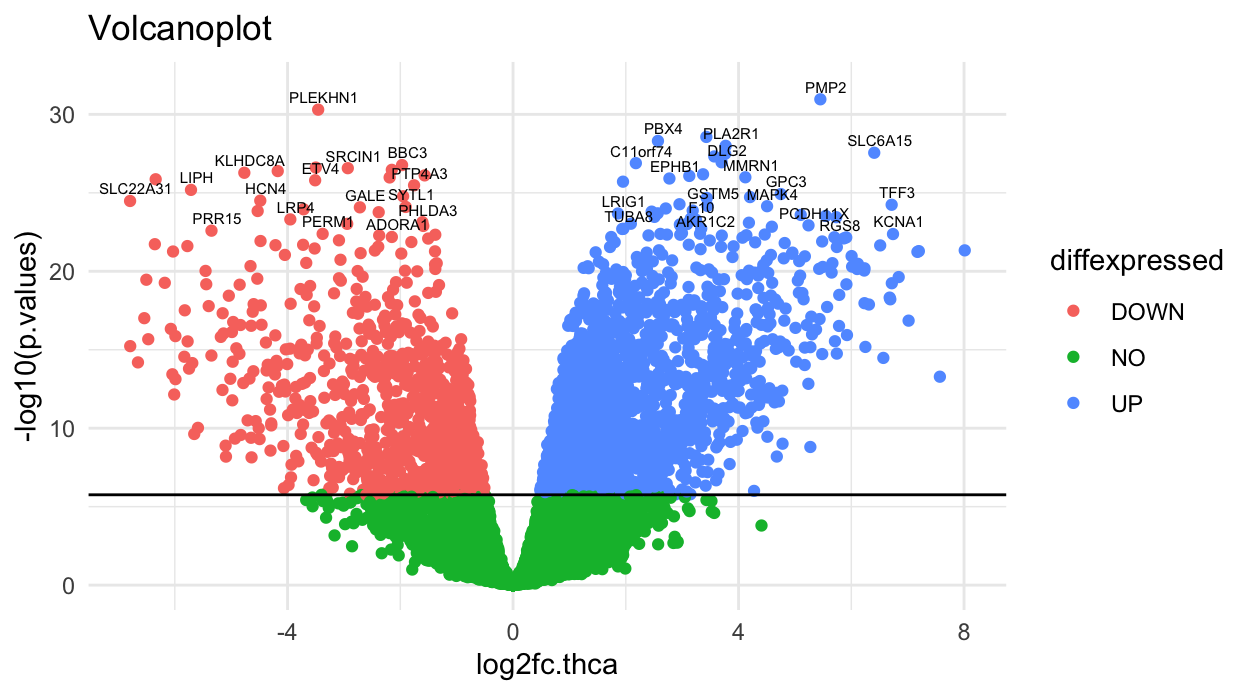
\includegraphics[width=0.9\linewidth]{figures/Volcanoplot} 

}

\caption{\textbf{Volcano plot of THCA expression data.} Downregulated genes are colored red, upregulated genes blue. Not significantly altered genes are colored green. Most significantly altered genes are labelled with their gene symbol}\label{fig:showvolcanoplot}
\end{figure}

\hypertarget{pan-cancer-analysis}{%
\section{Pan cancer analysis}\label{pan-cancer-analysis}}

\textbf{GSVA of TCGA expression data reveals four clusters of cancer
types.} A pathway activity matrix was computed as described in methods
section. The obtained pathway activity matrix was visualized as a
heatmap. (Figure \ref{fig:meanexp} and supplementary material figure
\ref{fig:exp}) The tumor types were clustered hierarchically based on
their mean pathway activity and formed four clusters correlating with
their histological type. The first cluster contains mainly
adenocarcinomas, while the second one contains predominately
glioblastomas. Leukemias are found only in the third cluster, and the
last cluster is enriched with sarcomas and carcinomas. Melanomas appear
in the second and fourth clusters. Furthermore, three observations were
made regarding specific information about pathway activity. Pathways,
which are important for nucleus import and export like the Ran shuttle
pathway, as well as pathways for transcription regulators in embryonic
stem cells are downregulated in glioblastoma and adenocarcinoma.
However, these pathways are upregulated in all other histological types.
Another observation is the clustering of glioblastoma. Pathways
initiating neurogenesis and pathways linked to differentiation of the
neural crest are upregulated only in glioblastoma (Wang \emph{et al.},
2021). Two other pathways, that are upregulated in glioblastoma cells
are pathways linked to the activity of tyrosine kinases. The
upregulation of tyrosine kinases promotes cell growth and proliferation
(Alberts and Walter, 2015). Taken together these two observations are in
line with the expected high proliferation rate commonly found in
glioblastoma. The third cluster is mainly related to adenocarcinomas,
more specifically liver hepatocellular carcinoma (LIHC), kidney renal
papillary cell carcinoma (KICH) and kidney renal clear cell carcinoma
(KIRC). The upregulated pathways are involved in the metabolism of
carbohydrates, synthesis of lipids, synthesis of amino acids and
detoxification.

\begin{figure}

{\centering 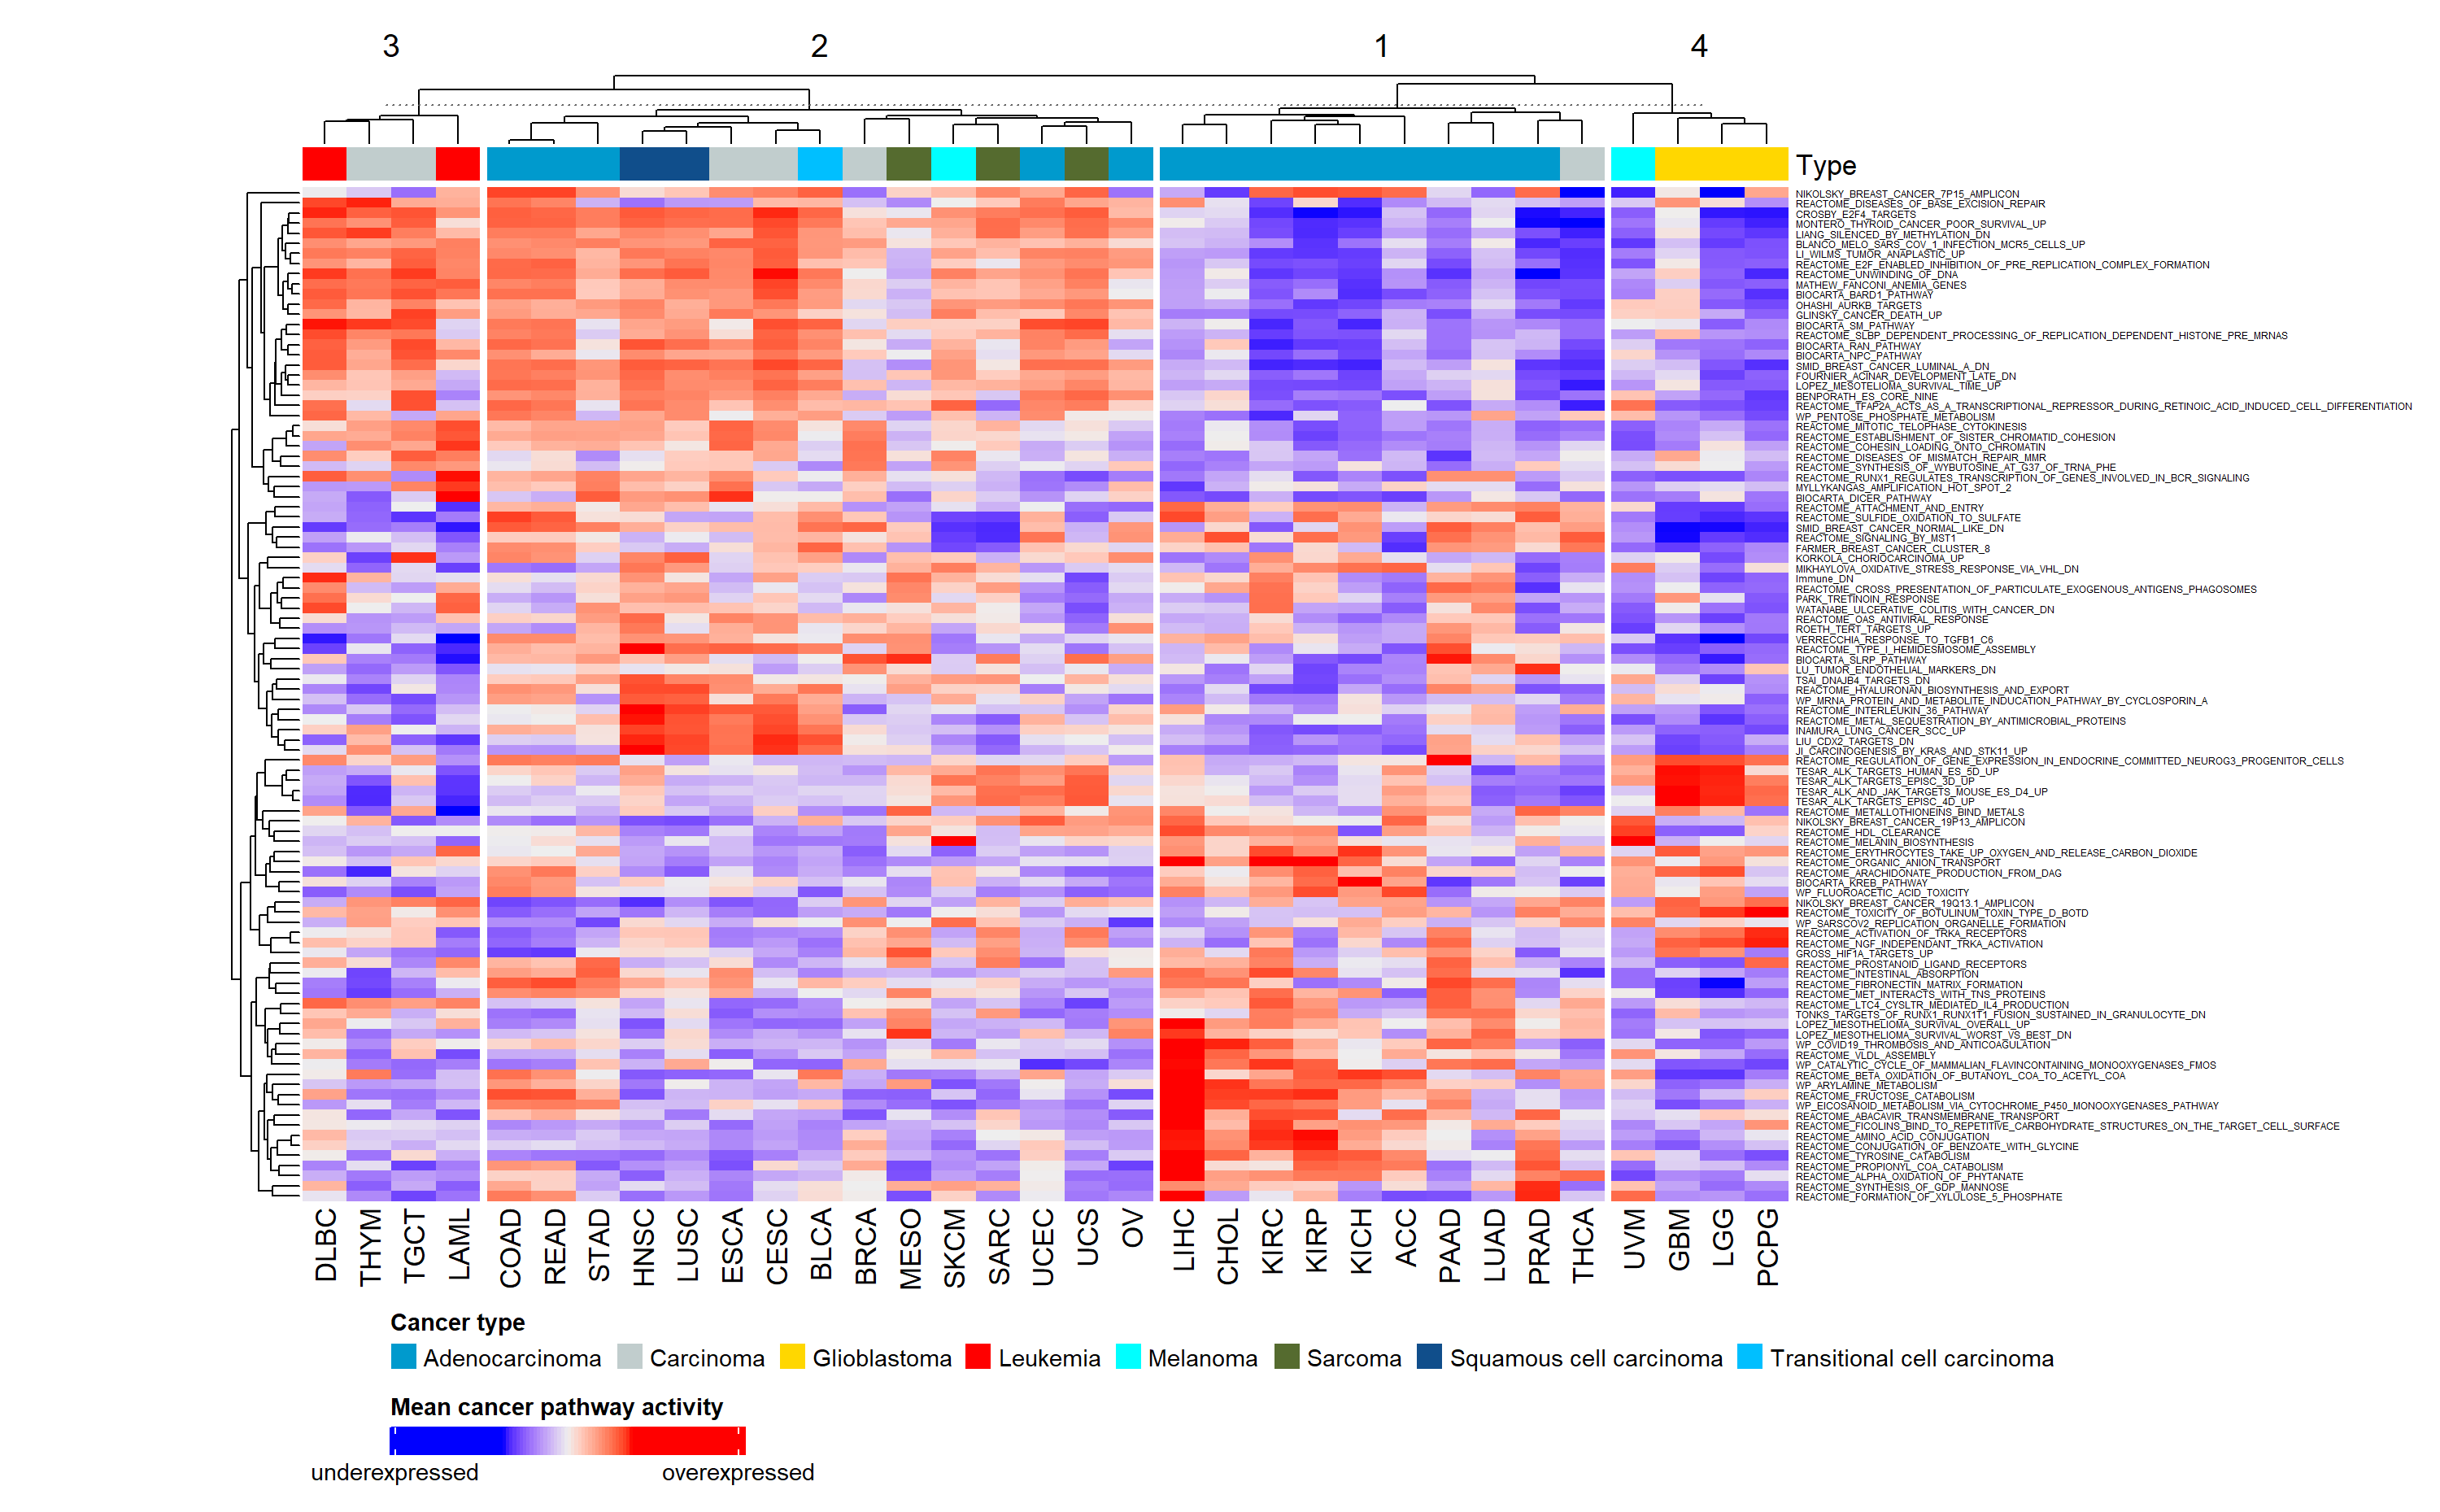
\includegraphics[width=0.87\linewidth]{figures/Pan Cancer mean expression top 100 pathways} 

}

\caption{\textbf{Mean pathway activity of the 100 most variant pathways for each tumor type.} Column clusters were obtained by complete hierachical clustering and subsequently split into four groups. Pathway activities were computed via GSVA of pan-cancer expression data. For all pathway activities see figure 6.2.}\label{fig:meanexp}
\end{figure}

\textbf{Dimension reduction of GSVA pan-cancer data reveals clusters in
pathway activity.} PCA was performed on GSVA pan-cancer data for UMAP
analysis. No apparent clustering was observed in the PCA data
(Supplementary material figure \ref{fig:PCAcancerform}). Subsequent UMAP
analysis, showed clear clusters for most cancer types. (Figure
\ref{fig:UMAPPanType} and supplementary material figure
\ref{fig:UMAPPanForm}). This complements the results obtained from our
heatmap and reassures, that the tumor types have characteristic pathway
activities. However, some cancers clustered better with their
histological type rather than tumor type. This was observed mainly for
carcinomas like squamous cell carcinoma and transitional cell carcinoma,
as well as sarcoma, lung adenocarcinoma, and ovarian cancer. These are
the same histological types that proved difficult to cluster in the mean
GSVA of TCGA expression. The UMAP confirmes, that the histological type
of a tumor has a major impact on the patients' gene expression profile.
The same analysis was performed for gene expression activity instead of
pathway activity to check for the reliability of the results. Similar
clusters were observed, which confirms our results. See figure
\ref{fig:UMAPGenform} in the supplementary material.

\begin{figure}

{\centering 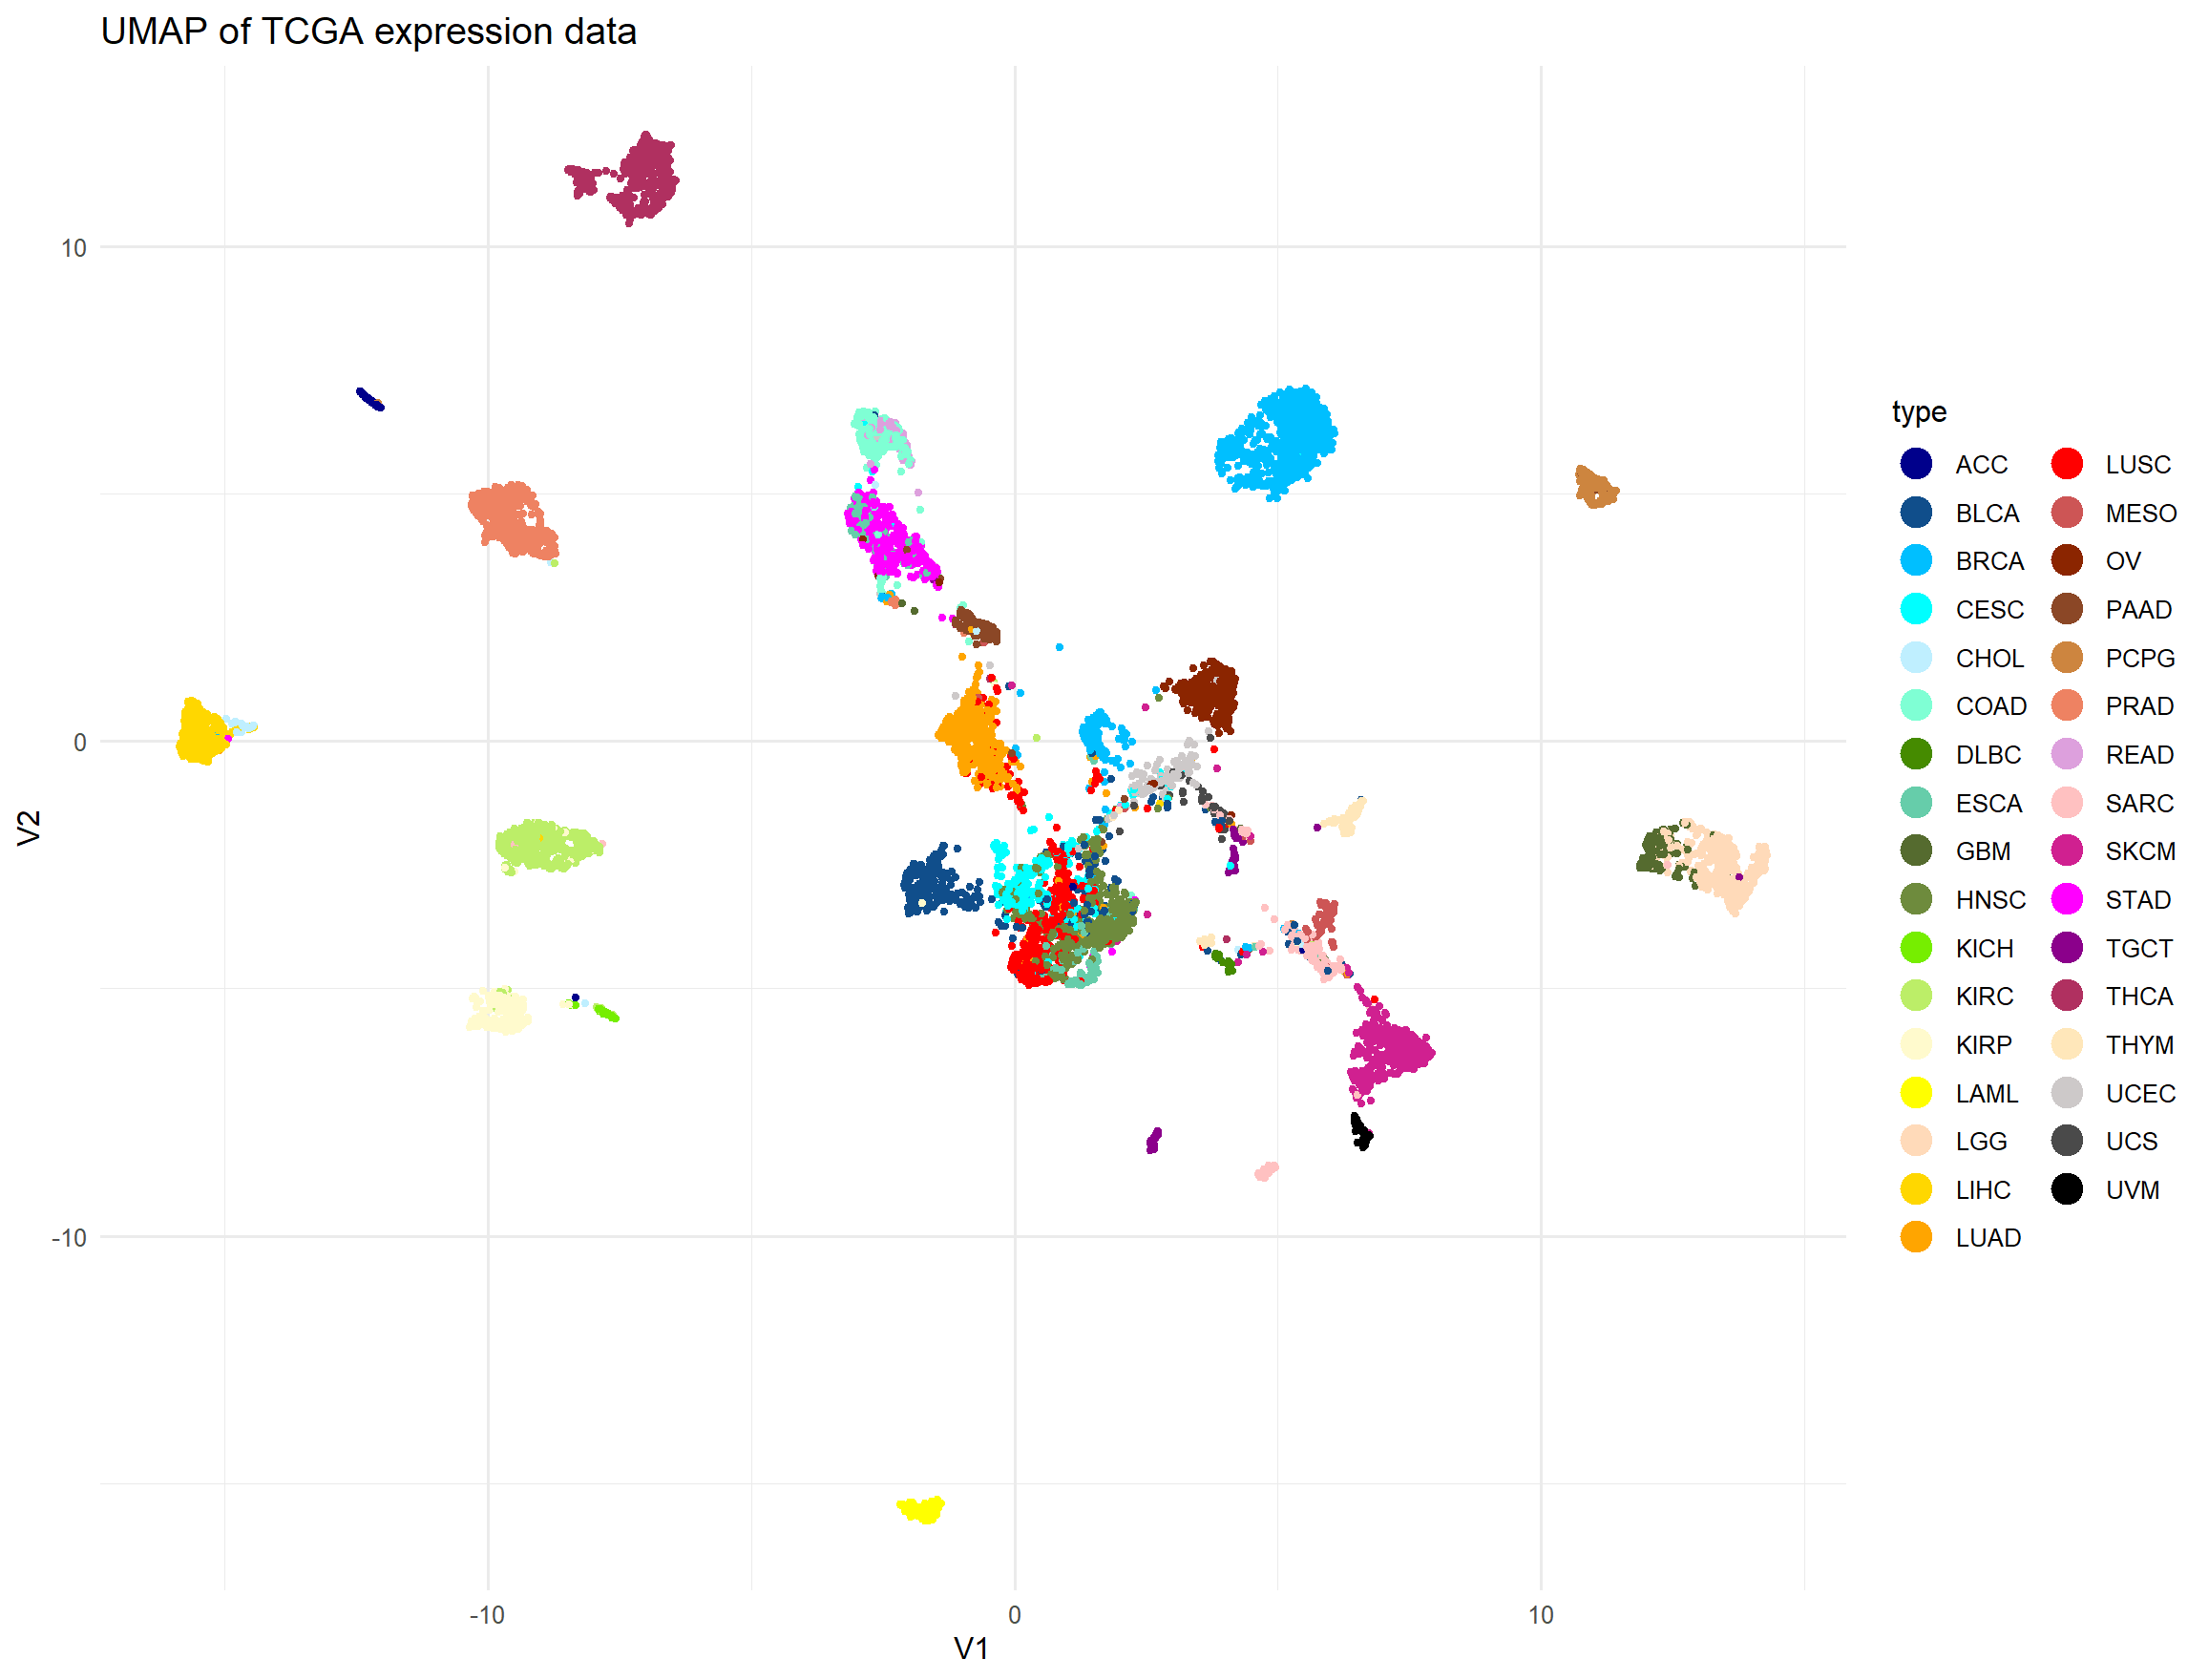
\includegraphics[width=0.8\linewidth]{figures/Pan Cancer UMAP} 

}

\caption{\textbf{UMAP of TCGA pathway activity.} Data points are colored by tumor type}\label{fig:UMAPPanType}
\end{figure}

\hypertarget{focused-analysis}{%
\section{Focused analysis}\label{focused-analysis}}

\textbf{GSVA on THCA expression data reveals pathways driving thyroid
carcinogenesis.} To grasp a general overview of the differences in
pathway activity between THCA and homeostatic thyroid tissue, GSVA was
performed for the THCA expression data. Based on the GSVA results,
altered pathways were identified using the workflow described for
volcano plots \ref{fig:THCAvolcano}. Most prominently among them were
pathways linked to proliferative signaling, such as upregulation of p53
inhibitory proteins and hedgehog pathway activating Gli proteins.
Further, the alpha6beta4 integrin signaling pathway and associated
pathways such as IL-36 signaling and Typ I hemidesmosome synthesis were
significantly enhanced in THCA. Further, signaling through the
EWSR1/FLI1-fusion protein was upregulated significantly. Lastly, THCA
showed downregulation of non-histone protein methylation.

\begin{figure}

{\centering 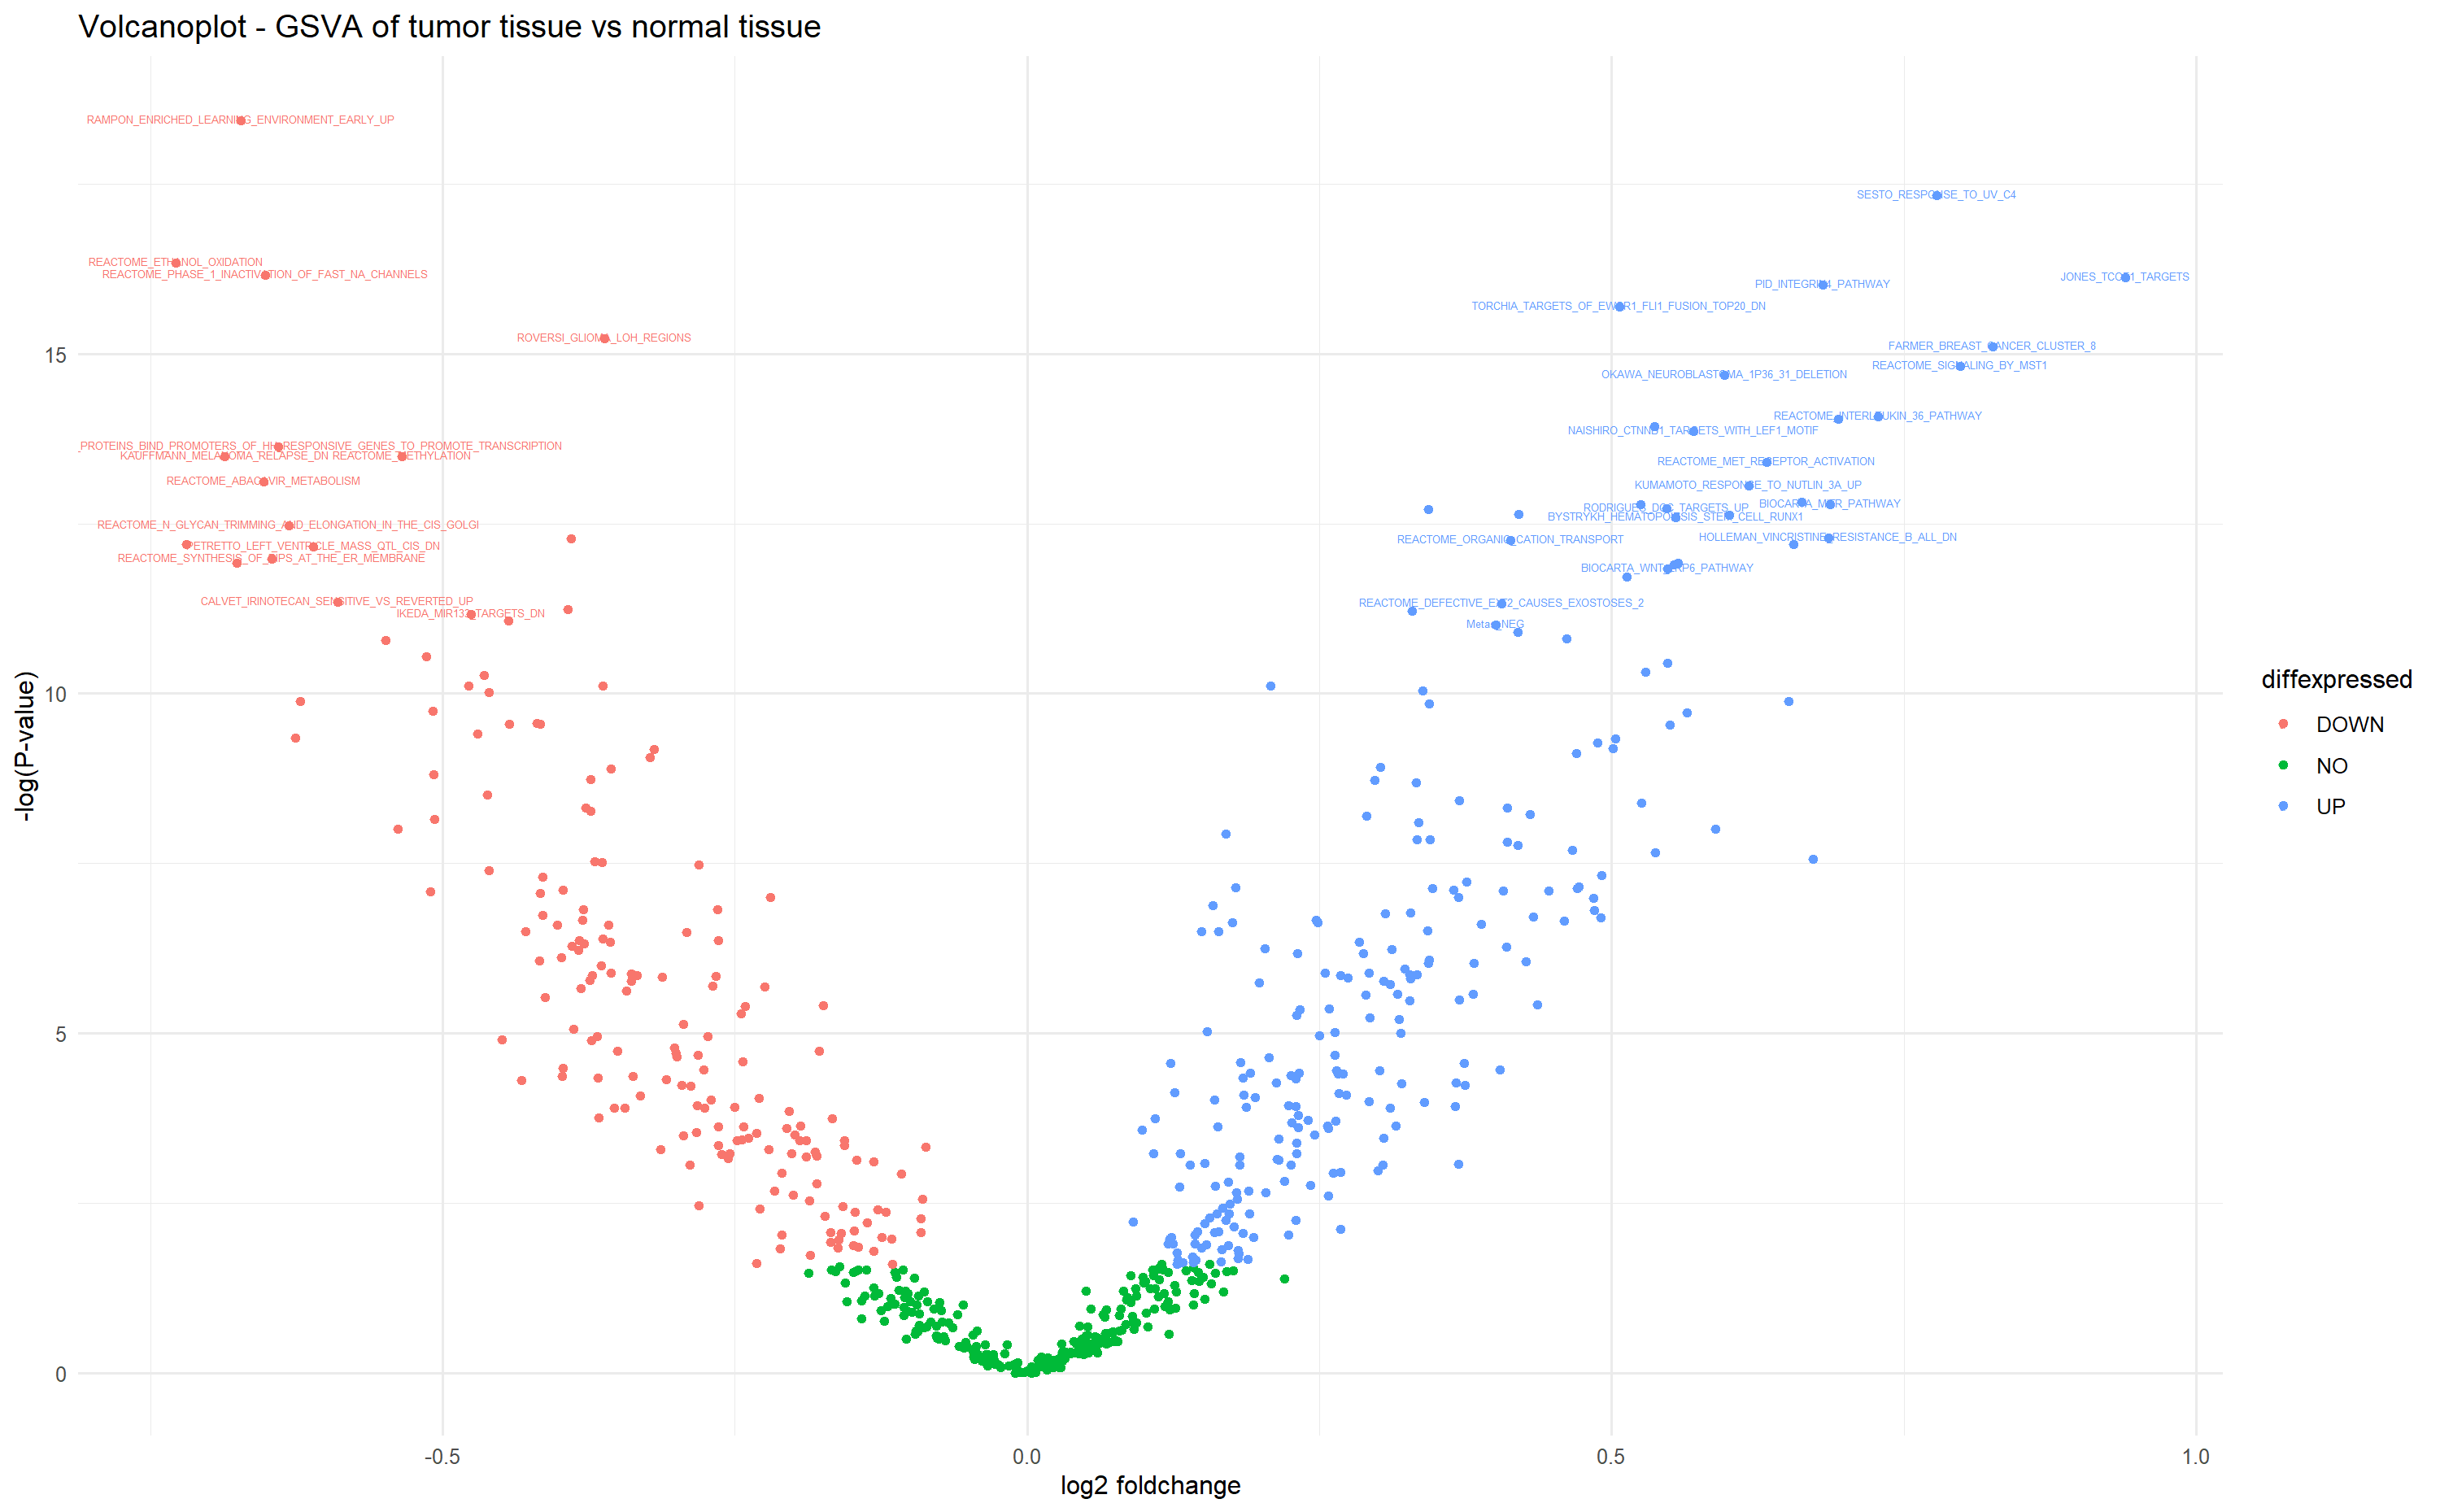
\includegraphics[width=0.8\linewidth]{figures/Volcanoplot THCA GSVA data} 

}

\caption{\textbf{Volcano plot of THCA pathway activity.} Downregulated pathways are colored red, upregulated pathways blue. Not significantly altered pathways are colored green. Most significantly altered pathways are labelled with their name.}\label{fig:THCAvolcano}
\end{figure}

\textbf{Pan-cancer data GSVA reveals three subtypes of THCA altering in
proliferative signaling.} To investigate potential subtypes of THCA, the
respective samples were taken from the pan-cancer GSVA data. The optimal
number of clusters was determined by an elbow plot and subsequent
k-means clustering revealed a total of three subtypes in THCA (Figure
\ref{fig:THCAhm}). This is consistent with the three clusters of THCA
observed in the full pan-cancer GSVA data. The follicular histological
type was enriched in cluster B, with no tall cell types present in this
cluster. Judging from histological type alone no difference in clusters
A and C was observed. Most significant changes in pathway activity were
observed in pathways concerning proliferative signaling. In comparison
with all other tumor types, cluster A displayed high activity of RAS,
JAK/STAT and EWSR1/FL1-fusion mediated signaling as well as elevated
signatures associated with carcinogenesis driven by alpha6beta4
activity. In contrast, these pathways were downregulated in cluster B,
with it showing elevated activity in mTOR, MAPK, PI3K, and EGFR
signaling cascades. Cluster C was found to upregulate all the
aforementioned forms of proliferative signaling. All clusters showed a
homogenous upregulation of hedgehog, ERBB2, and MST1 pathway activity.
Regarding immune response, cluster C showed no significant alterations
in the respective hallmark pathways, however, these pathways were
downregulated in both clusters A and B. With this data, we can identify
two seemingly different forms of proliferative signaling driving
carcinogenesis in THCA. These forms can either occur separately as in
the case of clusters A and B or combined as for cluster C.

\begin{figure}

{\centering 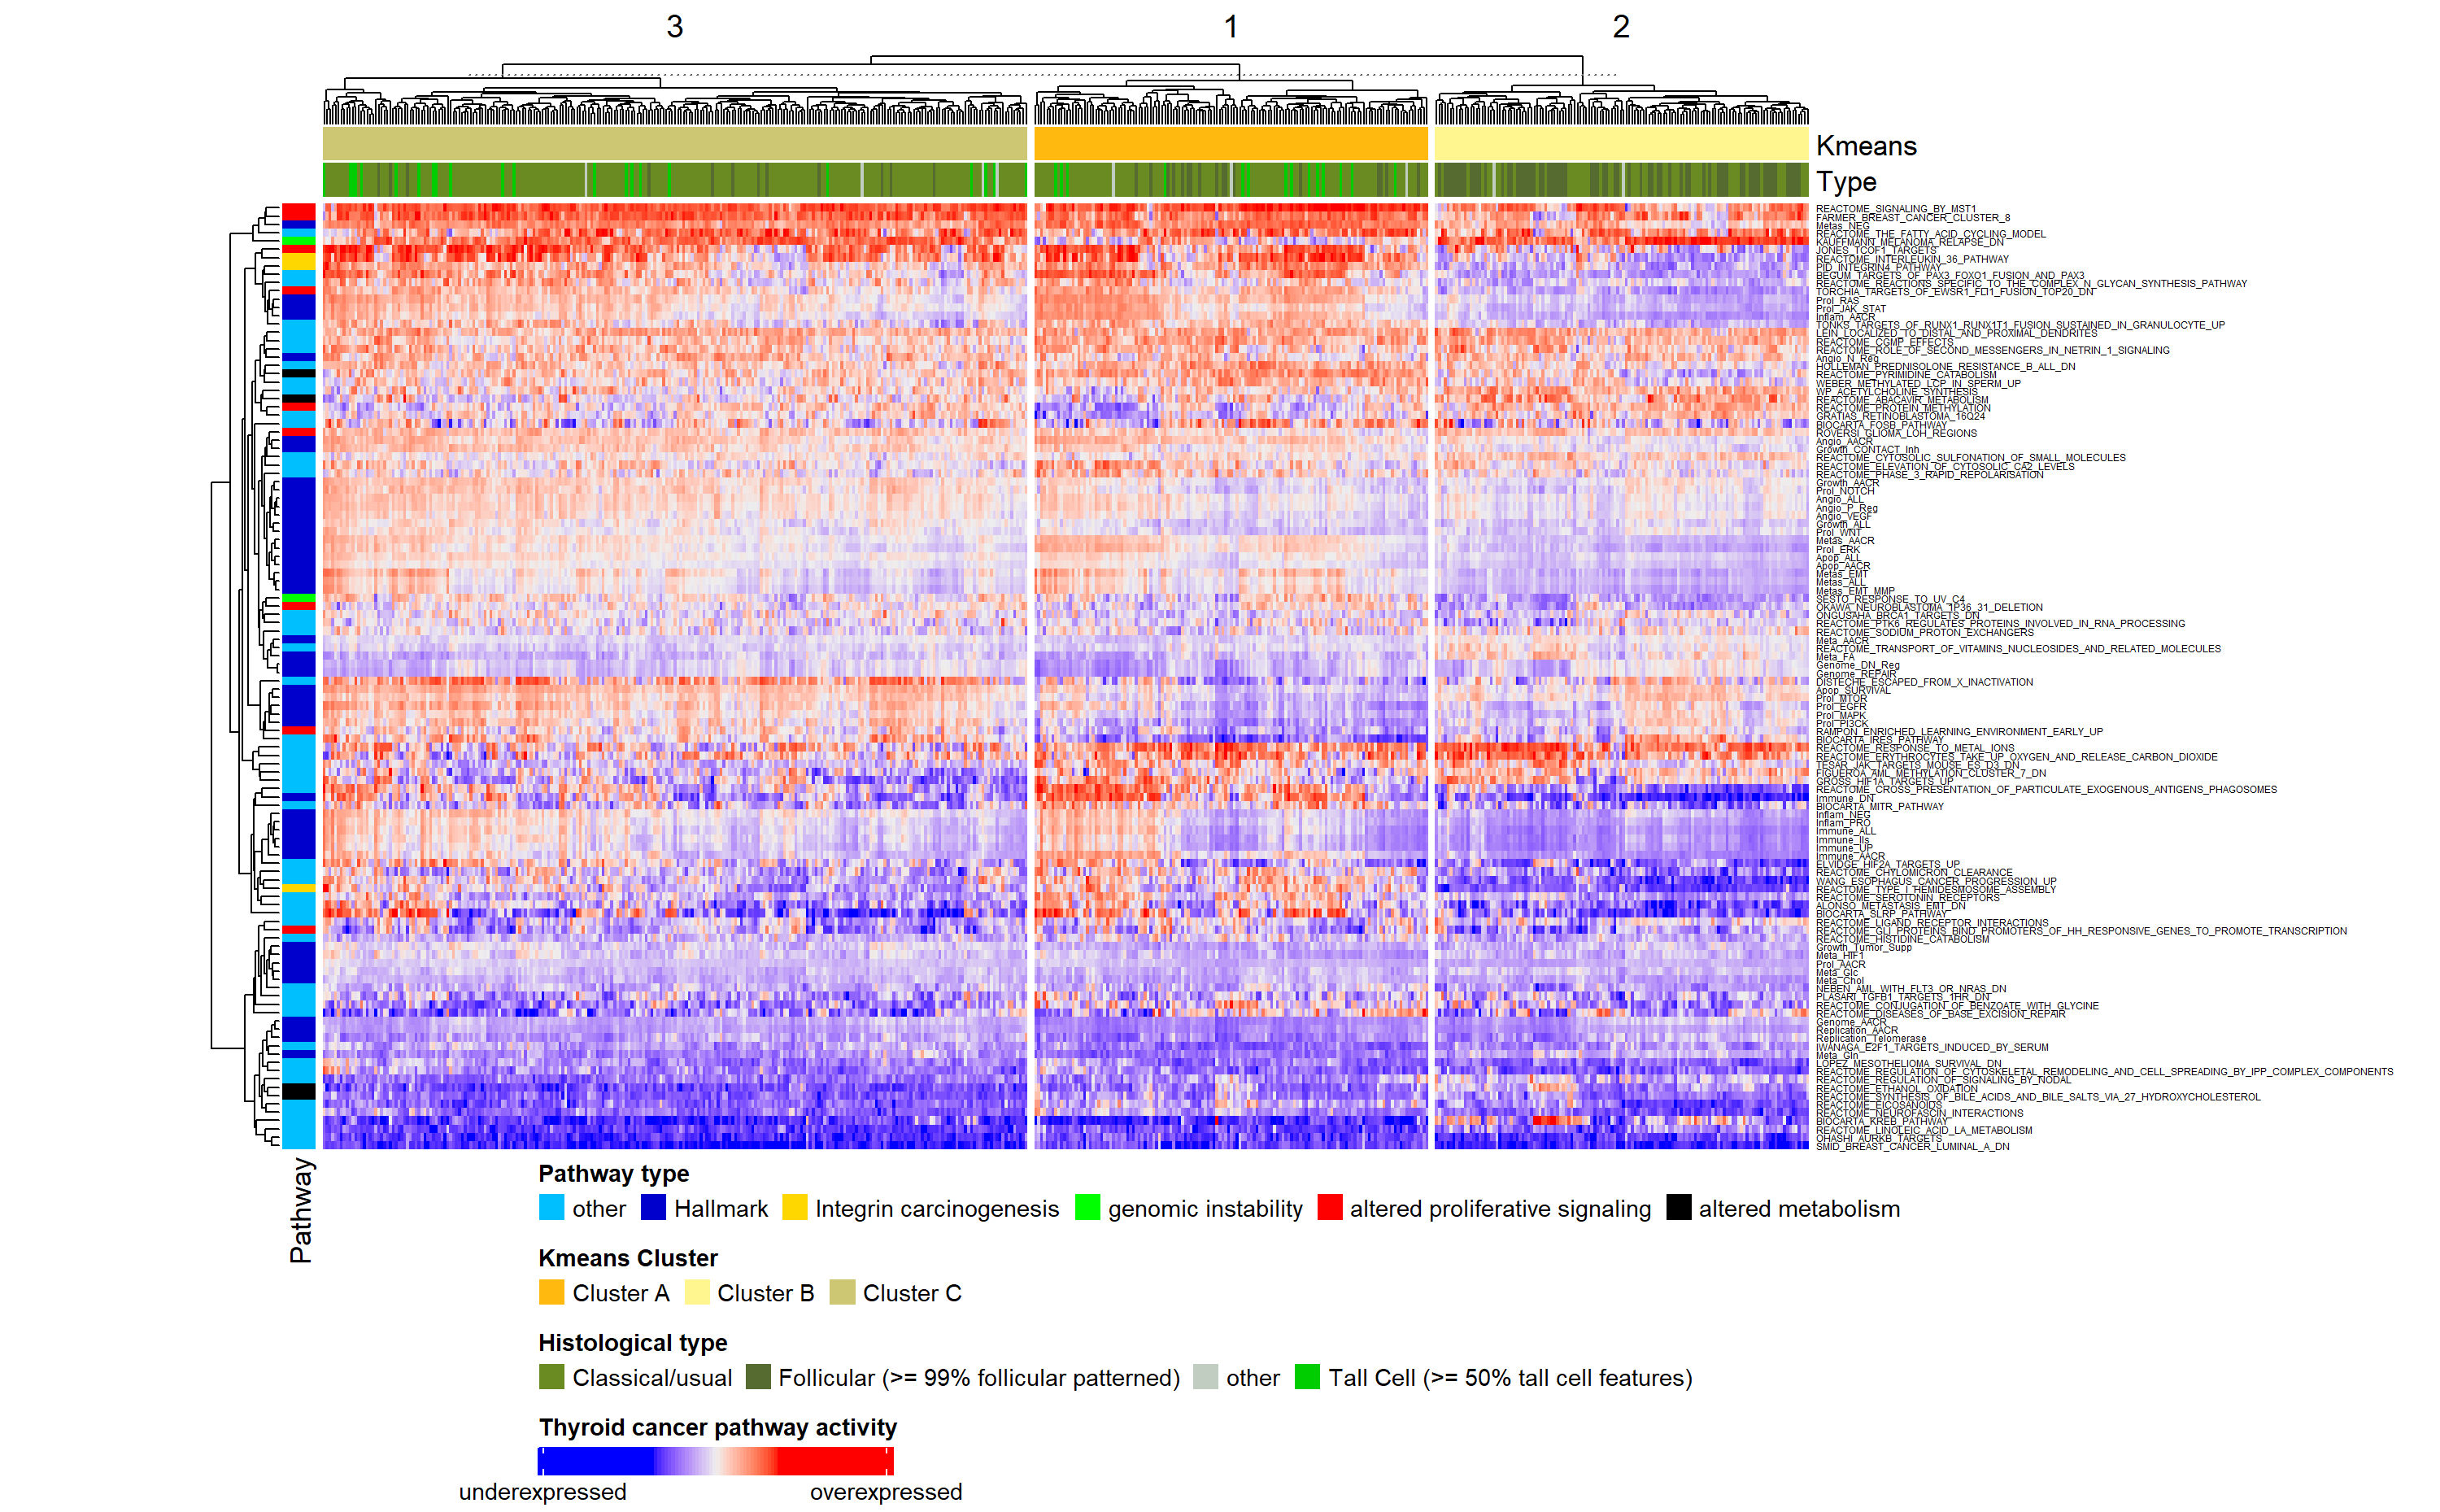
\includegraphics[width=0.9\linewidth]{figures/THCA Heatmap from Pancancer data top 50 pathways} 

}

\caption{\textbf{Pathway activity of the 50 most variant, hallmark, and 20 most significantly altered pathways for each patient.} Column clusters were obtained by k-means clustering with k=3. Pathway activities were computed via GSVA of pan-cancer expression data.}\label{fig:THCAhm}
\end{figure}

\textbf{THCA subtypes do not differ in their metabolism.} To investigate
how the identified subtypes compare to homeostatic thyroid tissue, GSEA
was performed for the THCA data. Consistent with the pan-cancer analysis
of THCA data, k-means clustering obtained three different clusters in
pathway activity -- verified as the optimal number of clusters via an
elbow plot. All clusters showed a similar change in metabolism
(Supplementary material figure \ref{fig:THCAhmGSEA}). Catabolic pathways
are downregulated whereas anabolic pathways e.g., fatty acid synthesis
show increased activity in comparison with normal tissue. Further, the
results seem consistent with the proliferative signaling activities
found previously. Alpha6beta4, RAS, JAK/STAT, and EWSR1/FL1-fusion
mediated signaling is upregulated in clusters one and three with low
expression in cluster two. However, the upregulation of mTOR, MAPK,
PI3K, and EGFR signaling in clusters two and three was observed only in
some samples. Regarding, immune response the expression profiles are
again consistent with differences observed in the GSVA pan-cancer data:
Both clusters one and two show a lower immune response compared to
cluster three. From these GSEA results, we can conclude that the three
subtypes of THCA differ in carcinogenesis and associated immune response
but share a similar metabolism consistent with the Warburg effect.

\hypertarget{regression-analysis-of-thca-pathway-activity}{%
\section{Regression analysis of THCA pathway
activity}\label{regression-analysis-of-thca-pathway-activity}}

To select a suitable pathway for regression analysis, the top 20\%
pathways regarding their variance in activity were chosen for the
regression model to predict. Pathways with little variance were found to
be better predicted by a null model. To factor in biological
significance, the intersect of the 25 most significantly altered
pathways from GSVA with the high variance pathways was computed. This
resulted in three significantly altered and highly variant pathways
among which the REACTOME\_INTERLEUKIN\_36\_PATHWAY (IL-36 pathway) was
selected. This gene set ranks 8th among the highest upregulated pathways
with an associated p-value of 8.411155e-15. Interleukin 36 signaling is
connected to both MAPK activity, through the activation of
NF-\(\kappa\)B and the expression of integrin alpha6beta4.(Bhatia
\emph{et al.}, 2013; Liberzon \emph{et al.}, 2015b; Queen \emph{et al.},
2019).

Regression of the IL-36 pathway gene set showed mixed results. After
multiple testing an architecture with two hidden layers with 10 and 20
neurons respectively at \texttt{set.seed(50)} was shown to produce the
best results for neuronal network regression. Among the tested models,
the neuronal network performed best on the test data with a mean squared
error (MSE) of 0.06. However, the linear regression model failed to
predict the data accurately (MSE = 0.62). Repeated linear regression
with just pathways contributing significantly to the result, the
performance was enhanced (MSE = 0.40), however, remained worse than a
null model (MSE~=~0.22) (Supplementary material figure \ref{fig:reg}). A
comparison of the MSE on the test and training data revealed, that the
linear model is highly overfitted (\(\Delta\)MSE~=~+0.55) with the
linear model with significant pathways fitting slightly better
(\(\Delta\)MSE~=~+0.23) to the data. Our null model displayed a good,
yet slightly underfitted performance with \(\Delta\)MSE~=~-0.08. With a
\(\Delta\)MSE~=~+0.009 the neuronal network shows an excellent fit.

A comparison of the four regression models via the F-test function
\texttt{var.test()} showed a significant improvement in the neuronal
network compared to all other models. All other models showed no
significant differences in their performance compared to each other.
(Supplementary material figure \ref{fig:reg}) From this data, we can
conclude that a neuronal network is the best choice for most accurately
predicting IL-36 pathway activity in our test data.

\hypertarget{discussion}{%
\chapter{Discussion}\label{discussion}}

Our pan-cancer analysis showed four clusters in pathway activity data.
We were able to find specific pathways, which were enriched only in
certain histological types like glioblastomas and adenocarcinomas. The
focused analysis of THCA expression data revealed pathways driving
carcinogenesis in Thyroid cancer. Furthermore, we were able to
subcategorize THCA into three subtypes based on proliferative signaling
pathway activity. As shown by the data signaling through alpha6beta4,
RAS, JAK/STAT, and EWSR1/FLI1-fusion mediated pathways are linked to the
non-follicular histological subtype of THCA. Our findings from
pan-cancer expression data show promising results. Via GSVA analysis, we
identified four clusters in the cancer types correlating strongly to the
associated histological type. Glioblastomas seem to take a special role
as they are predominantly characterized by the high activity of neural
crest differentiation pathways and receptor tyrosine kinases. This is in
line with previous studies showing that glioblastomas derive from neural
crest cells (Bednarczyk and McIntyre, 1992).

This was also found for some melanoma like UVM, which explains the
observed clustering of UVM with other glioblastomas. Also, the high
receptor tyrosine kinase activity has been linked to the formation of
UVM and glioblastoma and suggested as a possible target for therapy
(Wade \emph{et al.}, 2013; Jo \emph{et al.}, 2019).

Further, especially liver and kidney adenocarcinoma seemed to form a
strong subcluster within the other adenocarcinoma. They are
characterized by exceptionally high activity of metabolic pathways such
as carbohydrate metabolism, lipid, and amino acid synthesis. Again, this
change in metabolism was previously found in hepatocellular carcinoma
(Sangineto \emph{et al.}, 2020). Upregulation of these metabolic
pathways may lead to cell growth and proliferation, due to higher
metabolic activity, providing more biomass and energy.

The most significant classification we found was the clustering of tumor
types by their differentiation stage. Poorly differentiated tumors like
leukemia and squamous cell carcinoma show an upregulation of pathways
associated with embryonic stem cell-like expression signatures. In
contrast, highly differentiated tumors like most adenocarcinoma as well
as most glioblastoma show low activation of these gene sets. Such a
clustering by differentiation stage was previously described by
Ben-Porath \emph{et al.}. However, these findings cannot be verified
directly as provided annotation data did not contain information
regarding the differentiation stage (Ben-Porath \emph{et al.}, 2008).

From our GSEA and pan-cancer GSVA results, we identify two separate ways
of carcinogenesis in THCA. The follicular subtype upregulates
proliferative signaling through mTOR/PI3K and MAPK signaling pathways,
which goes along with previous studies Noh \emph{et al.} (2010).

The finding that the alpha6beta4 integrin signaling pathway and
associated pathways such as IL-36 signaling and Typ I hemidesmosome
synthesis were significantly enhanced in THCA is in line with previous
studies. Those studies link alpha6beta4 signaling to the development of
aggressive forms of thyroid cancer (Noh \emph{et al.}, 2010; Queen
\emph{et al.}, 2019). Also, oncogenic signaling pathways commonly
associated with different cancer types were significantly upregulated in
THCAs. Among them, we observed ERBB2 and MST1 signaling commonly found
in breast cancer. A role for MSP/Ron in breast cancer has recently been
elucidated, wherein this pathway regulates tumor growth, angiogenesis,
and metastasis (Kretschmann \emph{et al.}, 2010).

An important pathway upregulated in THCA is signaling through
EWSR1/FLI1-fusion protein, while non-histone protein methylation is
downregulated in THCA. This process was identified as an import
modulator of intracellular signaling by the MAPK, WNT, BMP, Hippo, and
JAK/STAT pathways and might play an important role as a driver of
carcinogenesis in THCA (Biggar and Li, 2015). Together these findings
give a general overview of mechanisms driving carcinogenesis in THCA.
However, no information about possible THCA subtypes or differences in
pathway activity between patients can be obtained from this data.

Pan-cancer GSVA shows three distinct clusters in the expression data,
upregulating either one or both ways of proliferative signaling. While
the follicular subtype seemed to strongly correlate with one cluster, a
similar process was not observed in tall-cell and classical phenotypes.
With more detailed annotation data it might be possible to link
anaplastic and papillary histological subtypes of THCA to the two yet
unassigned clusters.

Despite differences in proliferative signaling, all clusters share an
upregulated hedgehog signaling pathway which is consistent with the
literature (Hinterseher \emph{et al.}, 2014). Also, metabolic changes in
line with the Warburg effect were observed in all clusters.

For regression analysis by linear regression and a neural network the
IL-36 pathway was chosen since it is connected to both MAPK activity and
through the activation of NF-kB and also the expression of integrin
alpha6beta4. An effective regression might be crucial in finding
potentially druggable targets in combating THCA. Our data suggest that
our neuronal network is well suited to predict pathway activities from
GSEA data. The model shows an excellent fit to data and produces only
minor errors. However, both linear models struggle in predicting the
data accurately. This might be since GSEA pathway activity data usually
clusters into an up- and downregulated group with no values in between.
Since the IL-36 pathway also shows this problem, the two clusters might
produce larger correlation values that might impact the accuracy of the
regression coefficients and the intercept. Secondly, the correlation of
the residuals with the test data values did not approach zero, thus, our
linearity assumption is not met. Therefore, it can be concluded that a
linear regression model is not well suited to predict the IL-36 pathway
activity accurately.

\textbf{Conclusion and Outlook}

Taken together our results are in line with current research and allow
for the following hypothesis: The expression profile of a given cancer
type depends highly on its differentiation stage and its histological
type but little on the actual tumor type itself. Understanding how these
changes in expression link to mutational signatures might help in
developing druggable targets for therapy.

Our findings suggest THCA can be divided into three subtypes based on
which proliferative signaling pathway is active. These findings are in
line with previous studies.

Further ways of analysis could be the prediction of the histological
type of THCA as well as the way of carcinogenesis with a neuronal
network. This might be possible with a larger training data set as well
as more detailed and specified annotations. Furthermore, it might be
possible to link whole genome sequencing and methylation data to pathway
activity. In that way, one could suggest a suitable targeted therapy
option for a THCA patient based only on sequencing data from a small
biopsy sample.

\clearpage

\hypertarget{references}{%
\chapter{References}\label{references}}

\hypertarget{refs}{}
\begin{CSLReferences}{0}{0}
\leavevmode\vadjust pre{\hypertarget{ref-cell}{}}%
Alberts, J, B., and Walter, P (2015). Molecular biology of the cell, New
York: Garland science.

\leavevmode\vadjust pre{\hypertarget{ref-neuralcrest}{}}%
Bednarczyk, JL, and McIntyre, BW (1992). Expression and ligand-binding
function of the integrin alpha4beta1 (VLA-4) on neural-crest-derived
tumor cell lines. Clinical \& Experimental Metastasis 10, 281--290.

\leavevmode\vadjust pre{\hypertarget{ref-dis4}{}}%
Ben-Porath, I, Thomson, MW, Carey, VJ, Ge, R, Bell, GW, Regev, A, and
Weinberg, RA (2008). An embryonic stem cell-like gene expression
signature in poorly differentiated aggressive human tumors. Nat Genet
40, 499--507.

\leavevmode\vadjust pre{\hypertarget{ref-result7}{}}%
Bhatia, V, Mula, RV, and Falzon, M (2013). Parathyroid hormone-related
protein regulates integrin alpha6 and beta4 levels via transcriptional
and post-translational pathways. Exp Cell Res 319, 1419--1430.

\leavevmode\vadjust pre{\hypertarget{ref-dis6}{}}%
Bi, C-L, Zhang, Y-Q, Li, B, Guo, M, and Fu, Y-L (2019). Retracted:
MicroRNA-520a-3p suppresses epithelial--mesenchymal transition,
invasion, and migration of papillary thyroid carcinoma cells via the
JAK1-mediated JAK/STAT signaling pathway. Journal of Cellular Physiology
234, 4054--4067.

\leavevmode\vadjust pre{\hypertarget{ref-result1}{}}%
Biggar, KK, and Li, SSC (2015). Non-histone protein methylation as a
regulator of cellular signalling and function. Nature Reviews Molecular
Cell Biology 16, 5--17.

\leavevmode\vadjust pre{\hypertarget{ref-THCA}{}}%
Cabanillas, ME, McFadden, DG, and Durante, C (2016). Thyroid cancer.
Lancet 388, 2783--2795.

\leavevmode\vadjust pre{\hypertarget{ref-PCA_aggressive}{}}%
Coca-Pelaz, A et al. (2020). Papillary thyroid cancer-aggressive
variants and impact on management: A narrative review. Adv Ther 37,
3112--3128.

\leavevmode\vadjust pre{\hypertarget{ref-biomart}{}}%
Durinck, S, Spellman, PT, Birney, E, and Huber, W (2009). Mapping
identifiers for the integration of genomic datasets with the
r/bioconductor package biomaRt. Nature Protocols 4, 1184--1191.

\leavevmode\vadjust pre{\hypertarget{ref-neuralnet}{}}%
Fritsch, S, Guenther, F, and Wright, MN (2019). Neuralnet: Training of
neural networks.

\leavevmode\vadjust pre{\hypertarget{ref-dis5}{}}%
Furuya, F, Lu, C, Willingham, MC, and Cheng, S (2007). Inhibition of
phosphatidylinositol 3-kinase delays tumor progression and blocks
metastatic spread in a mouse model of thyroid cancer. Carcinogenesis 28,
2451--2458.

\leavevmode\vadjust pre{\hypertarget{ref-cancer_hallmarks}{}}%
Hanahan, D, and Weinberg, RA (2011). Hallmarks of cancer: The next
generation. Cell 144, 646--674.

\leavevmode\vadjust pre{\hypertarget{ref-GSVA}{}}%
Hänzelmann, S, Castelo, R, and Guinney, J (2013a). GSVA: Gene set
variation analysis for microarray and RNA-seq data. BMC Bioinformatics
14, 7.

\leavevmode\vadjust pre{\hypertarget{ref-gsva}{}}%
Hänzelmann, S, Castelo, R, and Guinney, J (2013b). {GSVA}: Gene set
variation analysis for microarray and {RNA-Seq} data. BMC
Bioinformatics.

\leavevmode\vadjust pre{\hypertarget{ref-seurat}{}}%
Hao, Y et al. (2021). Integrated analysis of multimodal single-cell
data. Cell 184, 3573--3587.e29.

\leavevmode\vadjust pre{\hypertarget{ref-dis8}{}}%
Hinterseher, U, Wunderlich, A, Roth, S, Ramaswamy, A, Bartsch, DK,
Hauptmann, S, Greene, BH, Fendrich, V, and Hoffmann, S (2014).
Expression of hedgehog signalling pathway in anaplastic thyroid cancer.
Endocrine 45, 439--447.

\leavevmode\vadjust pre{\hypertarget{ref-dis1}{}}%
Jo, DH, Kim, JH, and Kim, JH (2019). Targeting tyrosine kinases for
treatment of ocular tumors. Archives of Pharmacal Research 42, 305--318.

\leavevmode\vadjust pre{\hypertarget{ref-PCA3}{}}%
Kant, R, Davis, A, and Verma, V (2020). Thyroid nodules: Advances in
evaluation and management. Am Fam Physician 102, 298--304.

\leavevmode\vadjust pre{\hypertarget{ref-umap}{}}%
Konopka, T (2022). Umap: Uniform manifold approximation and projection.

\leavevmode\vadjust pre{\hypertarget{ref-fgsea}{}}%
Korotkevich, G, Sukhov, V, and Sergushichev, A (2019). Fast gene set
enrichment analysis. bioRxiv.

\leavevmode\vadjust pre{\hypertarget{ref-result2}{}}%
Kretschmann, KL, Eyob, H, Buys, SS, and Welm, AL (2010). The macrophage
stimulating protein/ron pathway as a potential therapeutic target to
impede multiple mechanisms involved in breast cancer progression. Curr
Drug Targets 11, 1157--1168.

\leavevmode\vadjust pre{\hypertarget{ref-msigdb}{}}%
Liberzon, A, Birger, C, Thorvaldsdóttir, H, Ghandi, M, Mesirov, JP, and
Tamayo, P (2015b). The molecular signatures database (MSigDB) hallmark
gene set collection. Cell Syst 1, 417--425.

\leavevmode\vadjust pre{\hypertarget{ref-integrin1}{}}%
Liberzon, A, Birger, C, Thorvaldsdóttir, H, Ghandi, M, Mesirov, JP, and
Tamayo, P (2015a). The molecular signatures database (MSigDB) hallmark
gene set collection. Cell Syst 1, 417--425.

\leavevmode\vadjust pre{\hypertarget{ref-PCA1}{}}%
Lin, JD (2007). Papillary thyroid carcinoma with lymph node metastases.
Growth Factors 25, 41--49.

\leavevmode\vadjust pre{\hypertarget{ref-lm}{}}%
Lunt, M (2013). Introduction to statistical modelling: Linear
regression. Rheumatology 54, 1137--1140.

\leavevmode\vadjust pre{\hypertarget{ref-tSNE}{}}%
Maaten, L van der, and Hinton, G (2008). Visualizing data using t-SNE.
Journal of Machine Learning Research 9, 2579--2605.

\leavevmode\vadjust pre{\hypertarget{ref-result3}{}}%
Noh, TW, Soung, YH, Kim, HI, Gil, HJ, Kim, JM, Lee, EJ, and Chung, J
(2010). Effect of {beta}4 integrin knockdown by RNA interference in
anaplastic thyroid carcinoma. Anticancer Res 30, 4485--4492.

\leavevmode\vadjust pre{\hypertarget{ref-dis7}{}}%
Oliveira, G, Polónia, A, Cameselle-Teijeiro, JM, Leitão, D, Sapia, S,
Sobrinho-Simões, M, and Eloy, C (2017). EWSR1 rearrangement is a
frequent event in papillary thyroid carcinoma and in carcinoma of the
thyroid with ewing family tumor elements (CEFTE). Virchows Archiv 470,
517--525.

\leavevmode\vadjust pre{\hypertarget{ref-result4}{}}%
Queen, D, Ediriweera, C, and Liu, L (2019). Function and regulation of
IL-36 signaling in inflammatory diseases and cancer development. Front
Cell Dev Biol 7, 317.

\leavevmode\vadjust pre{\hypertarget{ref-integrin2}{}}%
Rabinovitz, I, and Mercurio, AM (1996). The integrin alpha 6 beta 4 and
the biology of carcinoma. Biochem Cell Biol 74, 811--821.

\leavevmode\vadjust pre{\hypertarget{ref-PCA}{}}%
Reese, A (2019). Modern statistics for modern biology s. HolmesW. Huber
2019 cambridge cambridge university press xxiv + 382 pp., £ 49.99 ISBN
978‐1‐108‐70529‐5. Journal of the Royal Statistical Society: Series A
(Statistics in Society) 182, 1647--1647.

\leavevmode\vadjust pre{\hypertarget{ref-neuronal}{}}%
Riedmiller, MA Rprop - description and implementation details.

\leavevmode\vadjust pre{\hypertarget{ref-dis3}{}}%
Sangineto, M, Villani, R, Cavallone, F, Romano, A, Loizzi, D, and
Serviddio, G (2020). Lipid metabolism in development and progression of
hepatocellular carcinoma. Cancers 12, 1419.

\leavevmode\vadjust pre{\hypertarget{ref-UMAP}{}}%
Sharma, S, Quinn, D, Melenhorst, JJ, and Pruteanu-Malinici, I (2021).
High-dimensional immune monitoring for chimeric antigen receptor t cell
therapies. Current Hematologic Malignancy Reports 16, 112--116.

\leavevmode\vadjust pre{\hypertarget{ref-GSEA}{}}%
Subramanian, A et al. (2005). Gene set enrichment analysis: A
knowledge-based approach for interpreting genome-wide expression
profiles. Proc Natl Acad Sci U S A 102, 15545--15550.

\leavevmode\vadjust pre{\hypertarget{ref-dis2}{}}%
Wade, A, Robinson, AE, Engler, JR, Petritsch, C, James, CD, and
Phillips, JJ (2013). Proteoglycans and their roles in brain cancer. The
FEBS Journal 280, 2399--2417.

\leavevmode\vadjust pre{\hypertarget{ref-result6}{}}%
Wang, X, Pei, Z, Hossain, A, Bai, Y, and Chen, G (2021). Transcription
factor-based gene therapy to treat glioblastoma through direct neuronal
conversion. Cancer Biol Med 18, 860--874.

\leavevmode\vadjust pre{\hypertarget{ref-ggplot2}{}}%
Wickham, H (2016). ggplot2: Elegant graphics for data analysis,
Springer-Verlag New York.

\leavevmode\vadjust pre{\hypertarget{ref-rank}{}}%
Zyla, J, Marczyk, M, Weiner, J, and Polanska, J (2017). Ranking metrics
in gene set enrichment analysis: Do they matter? BMC Bioinformatics 18,
256.

\end{CSLReferences}

\clearpage

\hypertarget{supplementary-material}{%
\chapter{Supplementary material}\label{supplementary-material}}

\hypertarget{given-data}{%
\section{Given data}\label{given-data}}

For pan-cancer analysis, a gene expression data frame with normalized
and log2 transformed bulk RNA-seq expression data for 60,489 genes in
9741 patients with 33 different forms of cancer and clinical annotations
was used. The data was derived from The Cancer Genome Atlas (TCGA). For
the focused analysis, only THCA data consisting of three data frames was
used: The first two contain normalized, and log2 transformed bulk
RNA-seq expression data for 19,624 genes in 59 THCA patients for
carcinogenic and homeostatic tissue. The third data frame complements
the data with the respective clinical annotations. The last object
contains 46 pathways associated with the hallmarks of cancer in the form
of a list of vectors containing gene identifiers. To perform enrichment
analysis, all 6366 canonical pathways were selected from the Molecular
Signatures Database (MSigDB) (Liberzon \emph{et al.}, 2015b) with the
\texttt{msigdbr::msigdbr()} function. As not to introduce a bias during
enrichment analysis, the similarity of MSigDB pathways among themselves
as well as with the hallmark pathways was computed with the Jaccard
index. The pathways with a Jaccard index greater than a set threshold
were discarded.

\hypertarget{preprocessing-of-expression-data}{%
\section{Preprocessing of expression
data}\label{preprocessing-of-expression-data}}

All expression data were checked for missing values. Subsequently, low
variance filtering was performed for TCGA and THCA tumor expression
data. Genes with variances below a threshold were discarded to reduce
dimensionality. Next, biotype filtering was performed for pan-cancer and
THCA expression data to reduce dimensionality further. Only genes
sharing biotypes with the hallmark pathways were kept for the following
analysis. The biotypes of the genes were retrieved using the
\texttt{biomart::getBM()} function from the ``biomart'' package (Durinck
\emph{et al.}, 2009). Only MSigDB pathways in which over 99\% of their
respective genes were present in the filtered expression data were
selected as final pathways.

\hypertarget{additional-computational-methods}{%
\section{Additional Computational
Methods}\label{additional-computational-methods}}

A Principal component analysis (PCA) is used to alter the coordinates of
a given dataset to its eigenvectors. This matrix rotation results in a
new set of basis vectors called principal components (PCs) - the
eigenvectors - that are orthogonal and show little correlation. Sorting
the PCs by their associated eigenvalue, the PCs explaining the most
variance can easily be identified, as they have the highest eigenvalue.
By displaying the data set in a coordinate system span by the \(n\) most
variant PCs, the dimensionalty of the data set is reduced to
\(\mathbb{R}^n\) with the lowest loss in variance. (Reese, 2019)

Linear regression is a statistical model that uses measurable values to
predict an outcome. For this purpose, a linear function serves as basis
to build the linear regression equation (Lunt, 2013). The coefficients
for each variable are estimated by their correlation and slope with the
predicted parameter. Lastly, all coefficients as well as the intersect
are optimized for the data set with a least sum of squares method.

The Jaccard index is the intersection, divided by the union of two sets.
Therefore, it can be used to identify the similarity of the sets.

\hypertarget{additional-figures}{%
\section{Additional Figures}\label{additional-figures}}

\begin{figure}

{\centering 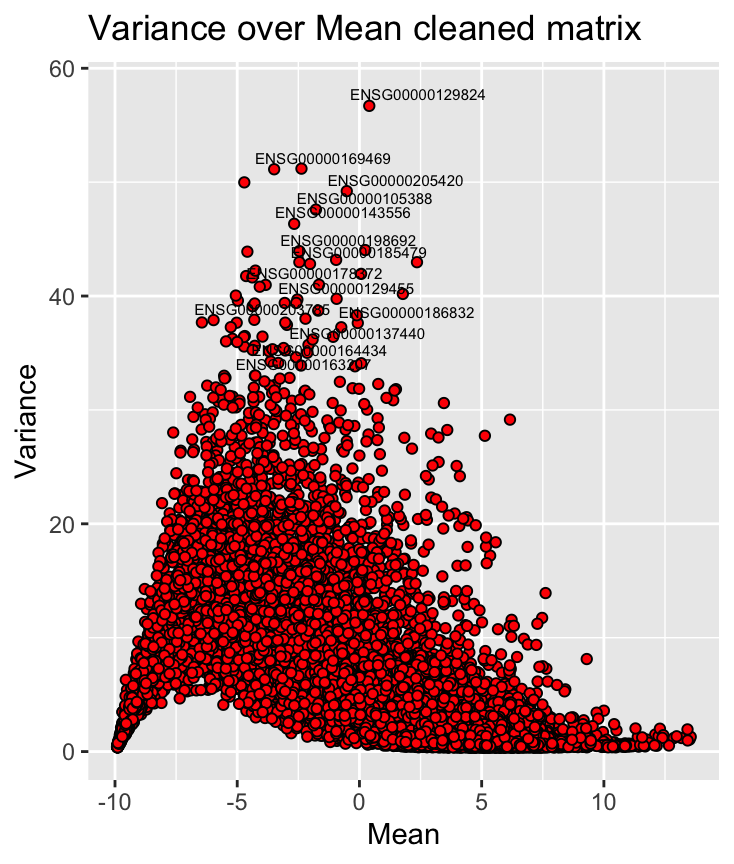
\includegraphics[width=0.65\linewidth]{figures/Variance_over mean_cleaned_matrix} 

}

\caption{\textbf{Mean-variance plot of cleaned TCGA expression data.} Y-axis shows variance of a gene expression, x-axis shows the log2 mean of a gene expression. Genes with variance greater 33 are labelled with their ENSEMBL-ID}\label{fig:showmeanvariance}
\end{figure}

\begin{figure}

{\centering 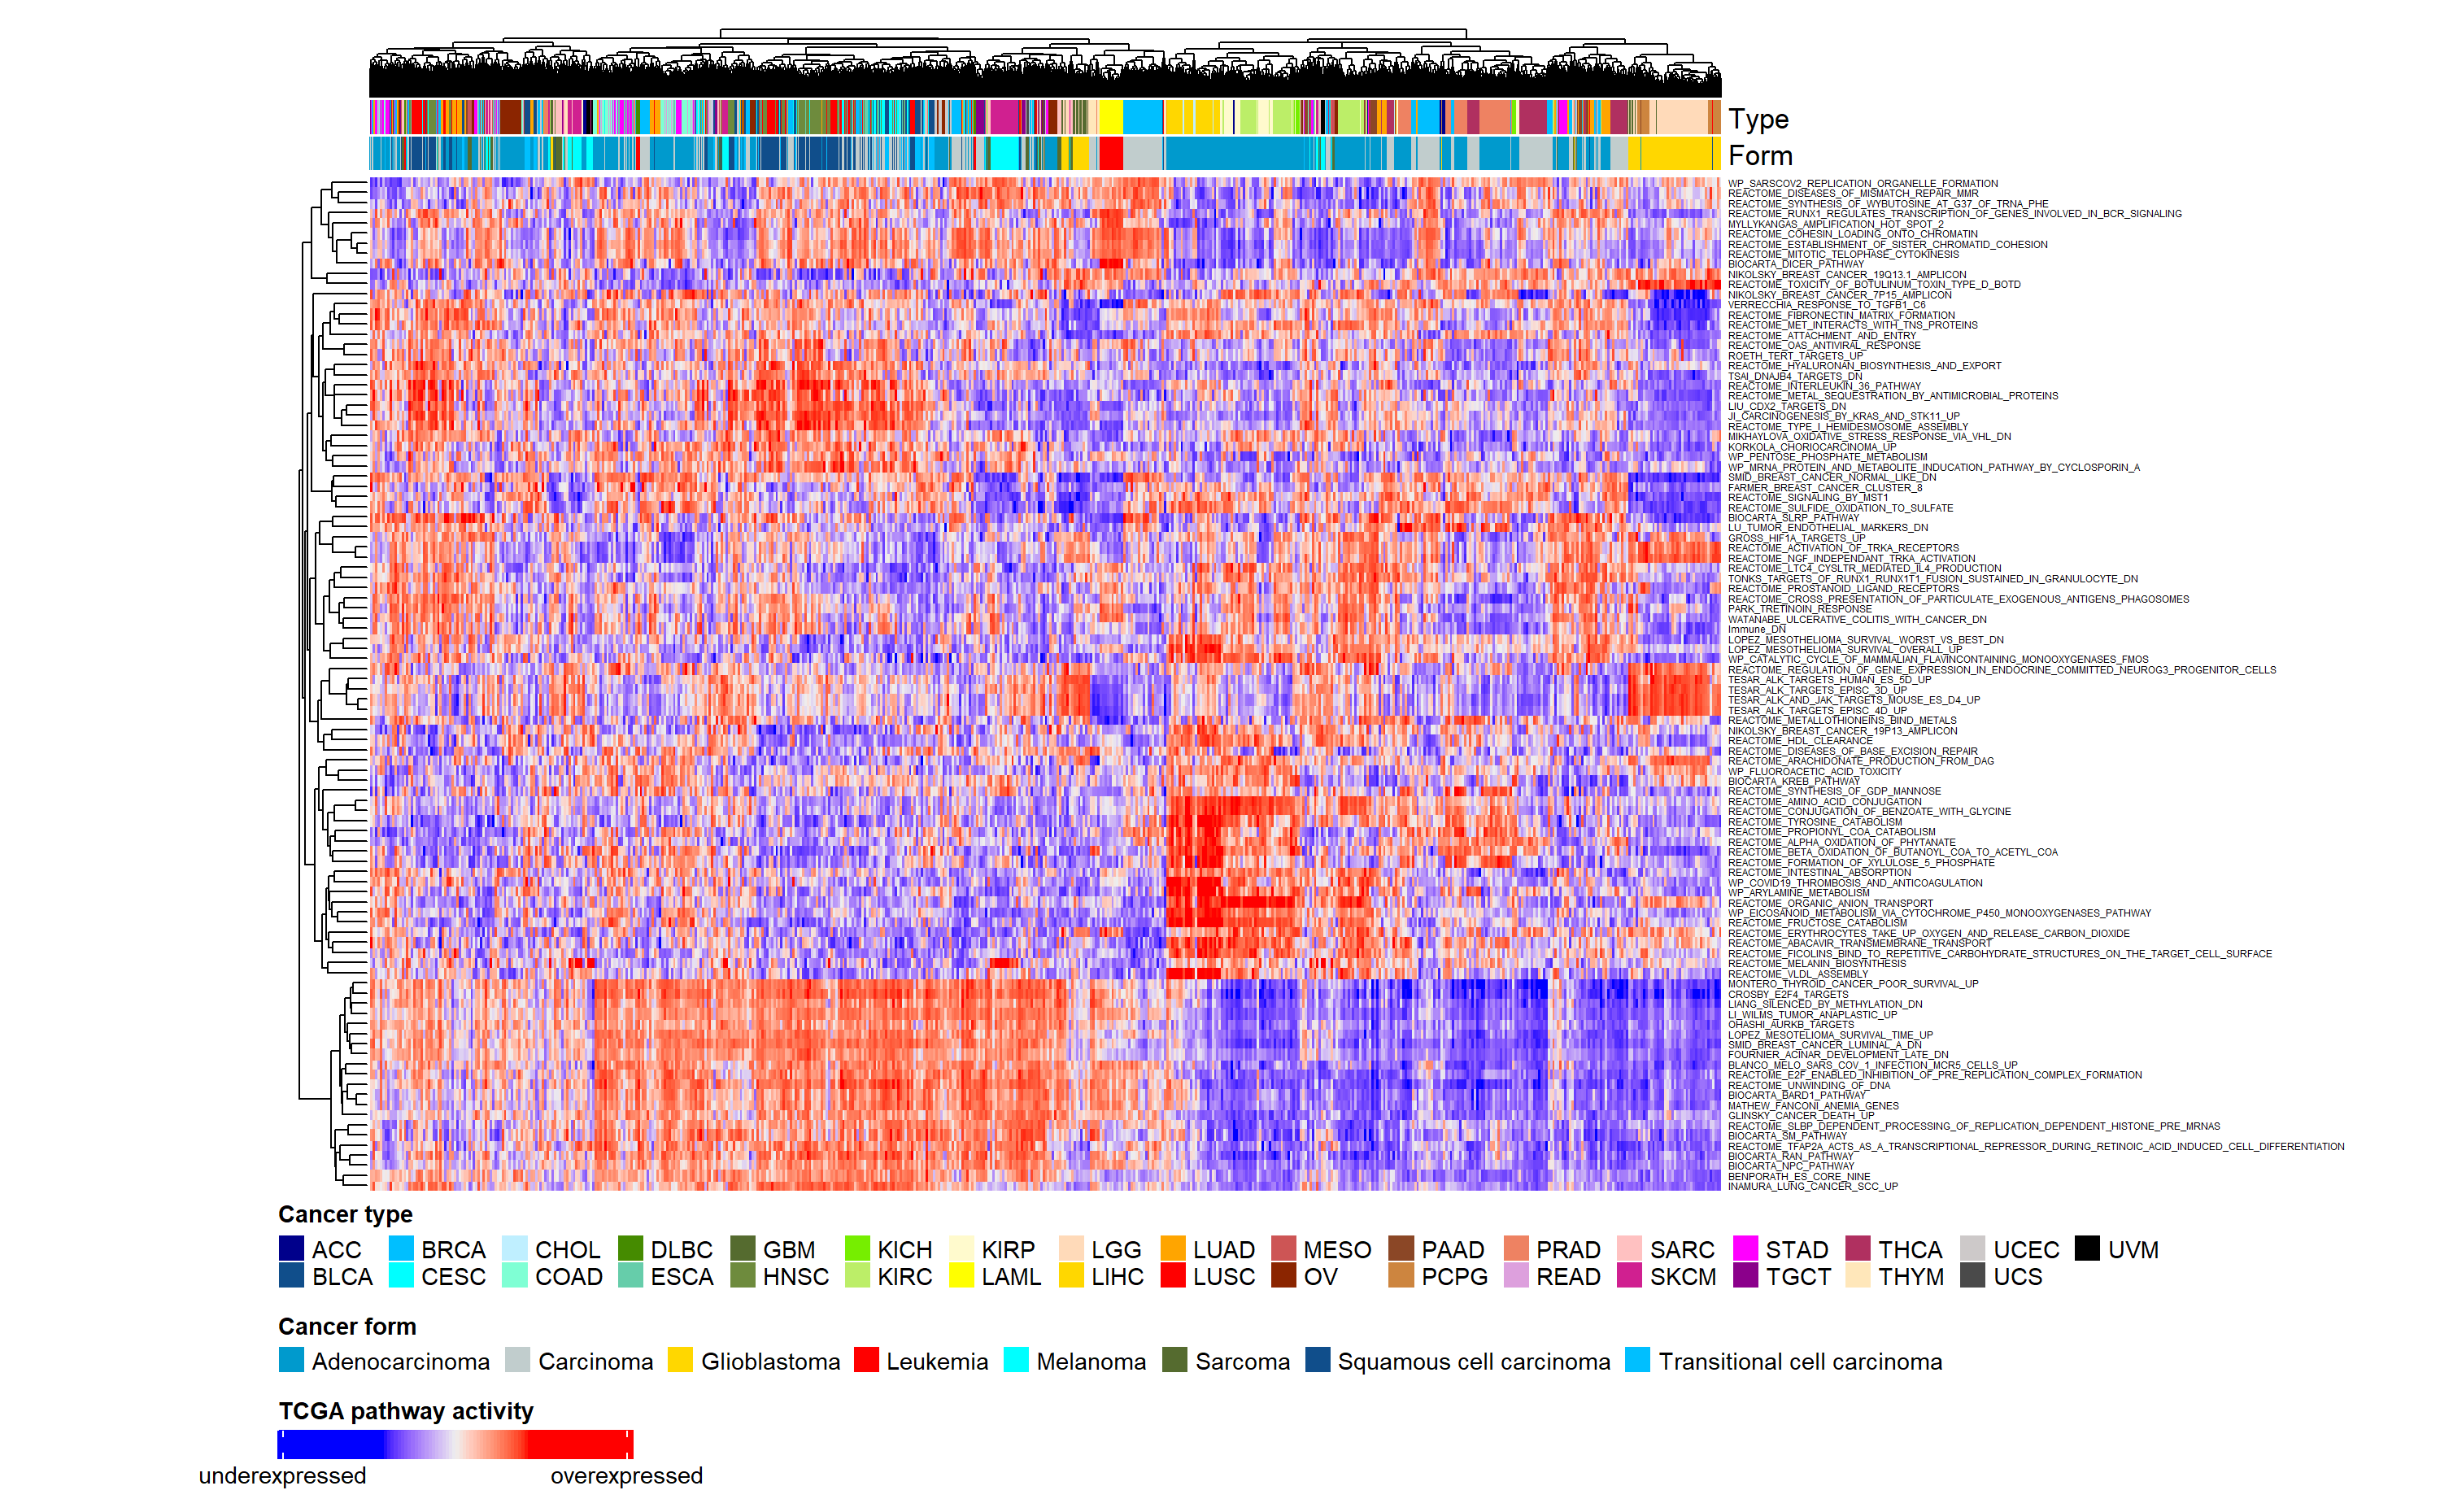
\includegraphics[width=1\linewidth]{figures/Pan Cancer GSVA Heatmap neu und fertig top 100 Pathways} 

}

\caption{\textbf{Pathway activity of the 100 most variant pathways for each patient.} Column and row clusters were obtained by complete hierachical clustering. Pathway activities were computed via GSVA of pan-cancer expression data. For all pathway activities see figure (XXX in the apendix).}\label{fig:exp}
\end{figure}

\begin{figure}

{\centering 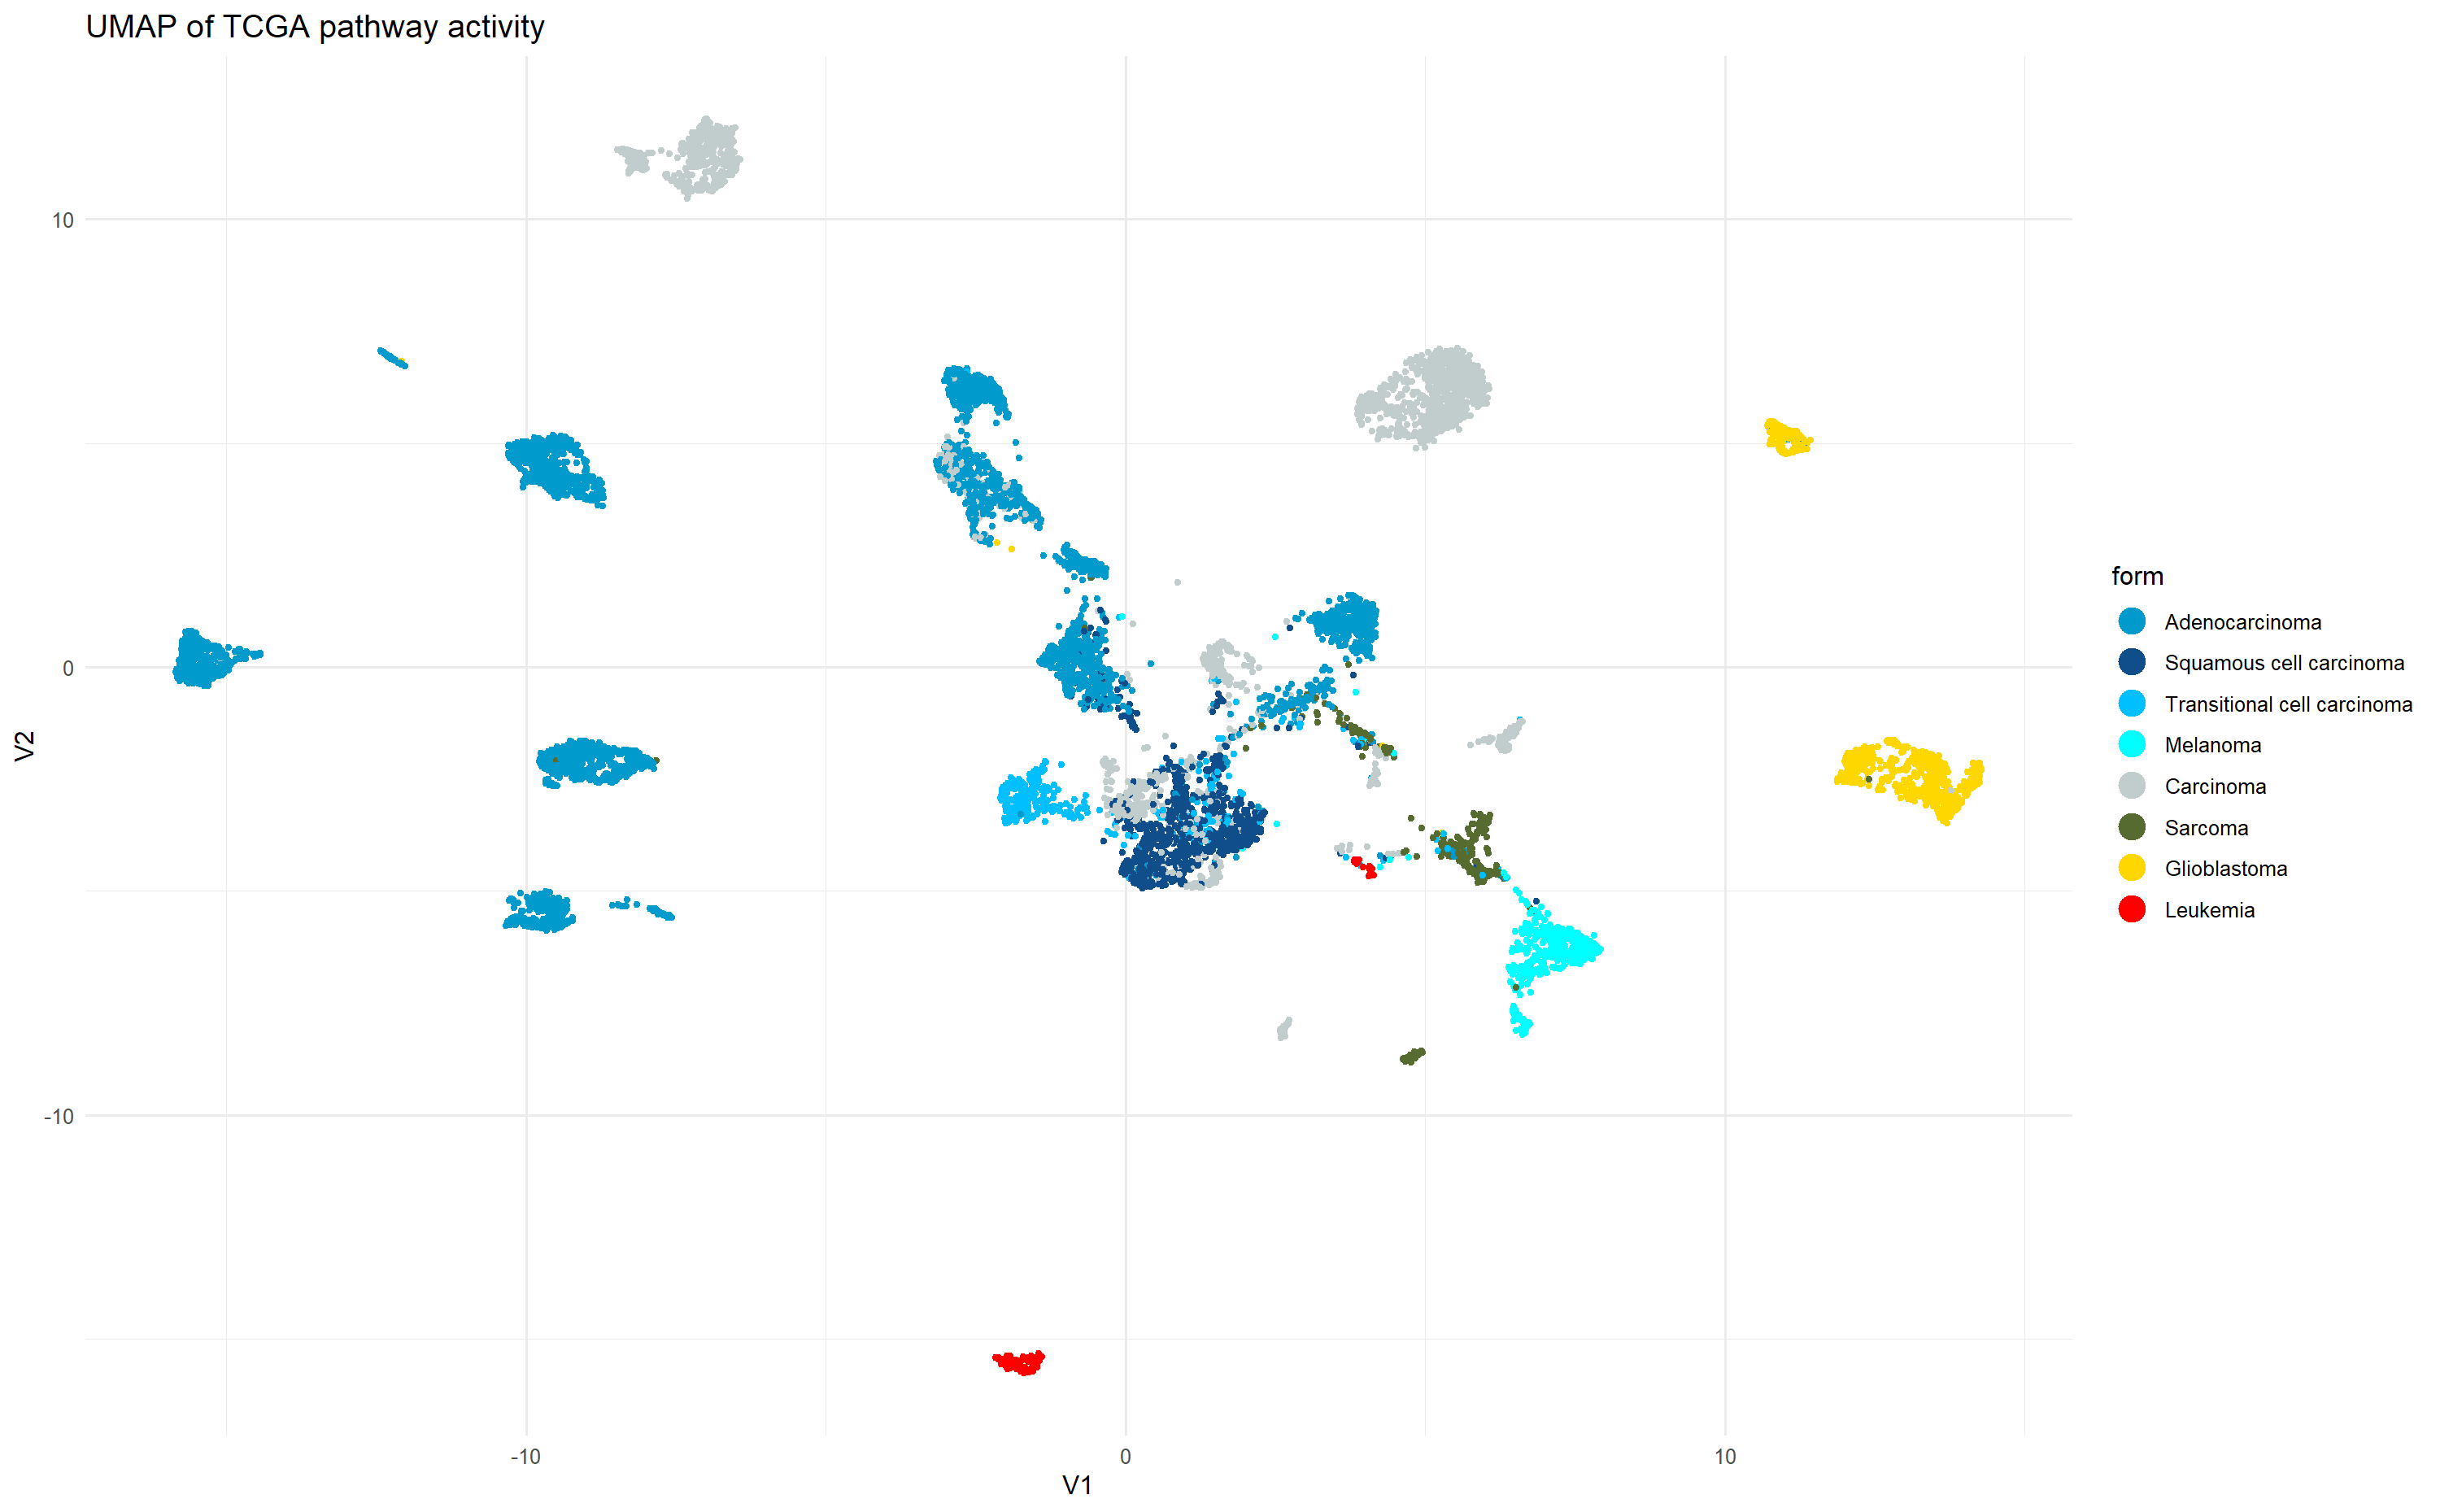
\includegraphics[width=0.8\linewidth]{figures/Pan Cancer UMAP cancer form} 

}

\caption{\textbf{UMAP of TCGA pathway activity,} colored by histological type}\label{fig:UMAPPanForm}
\end{figure}

\begin{figure}

{\centering 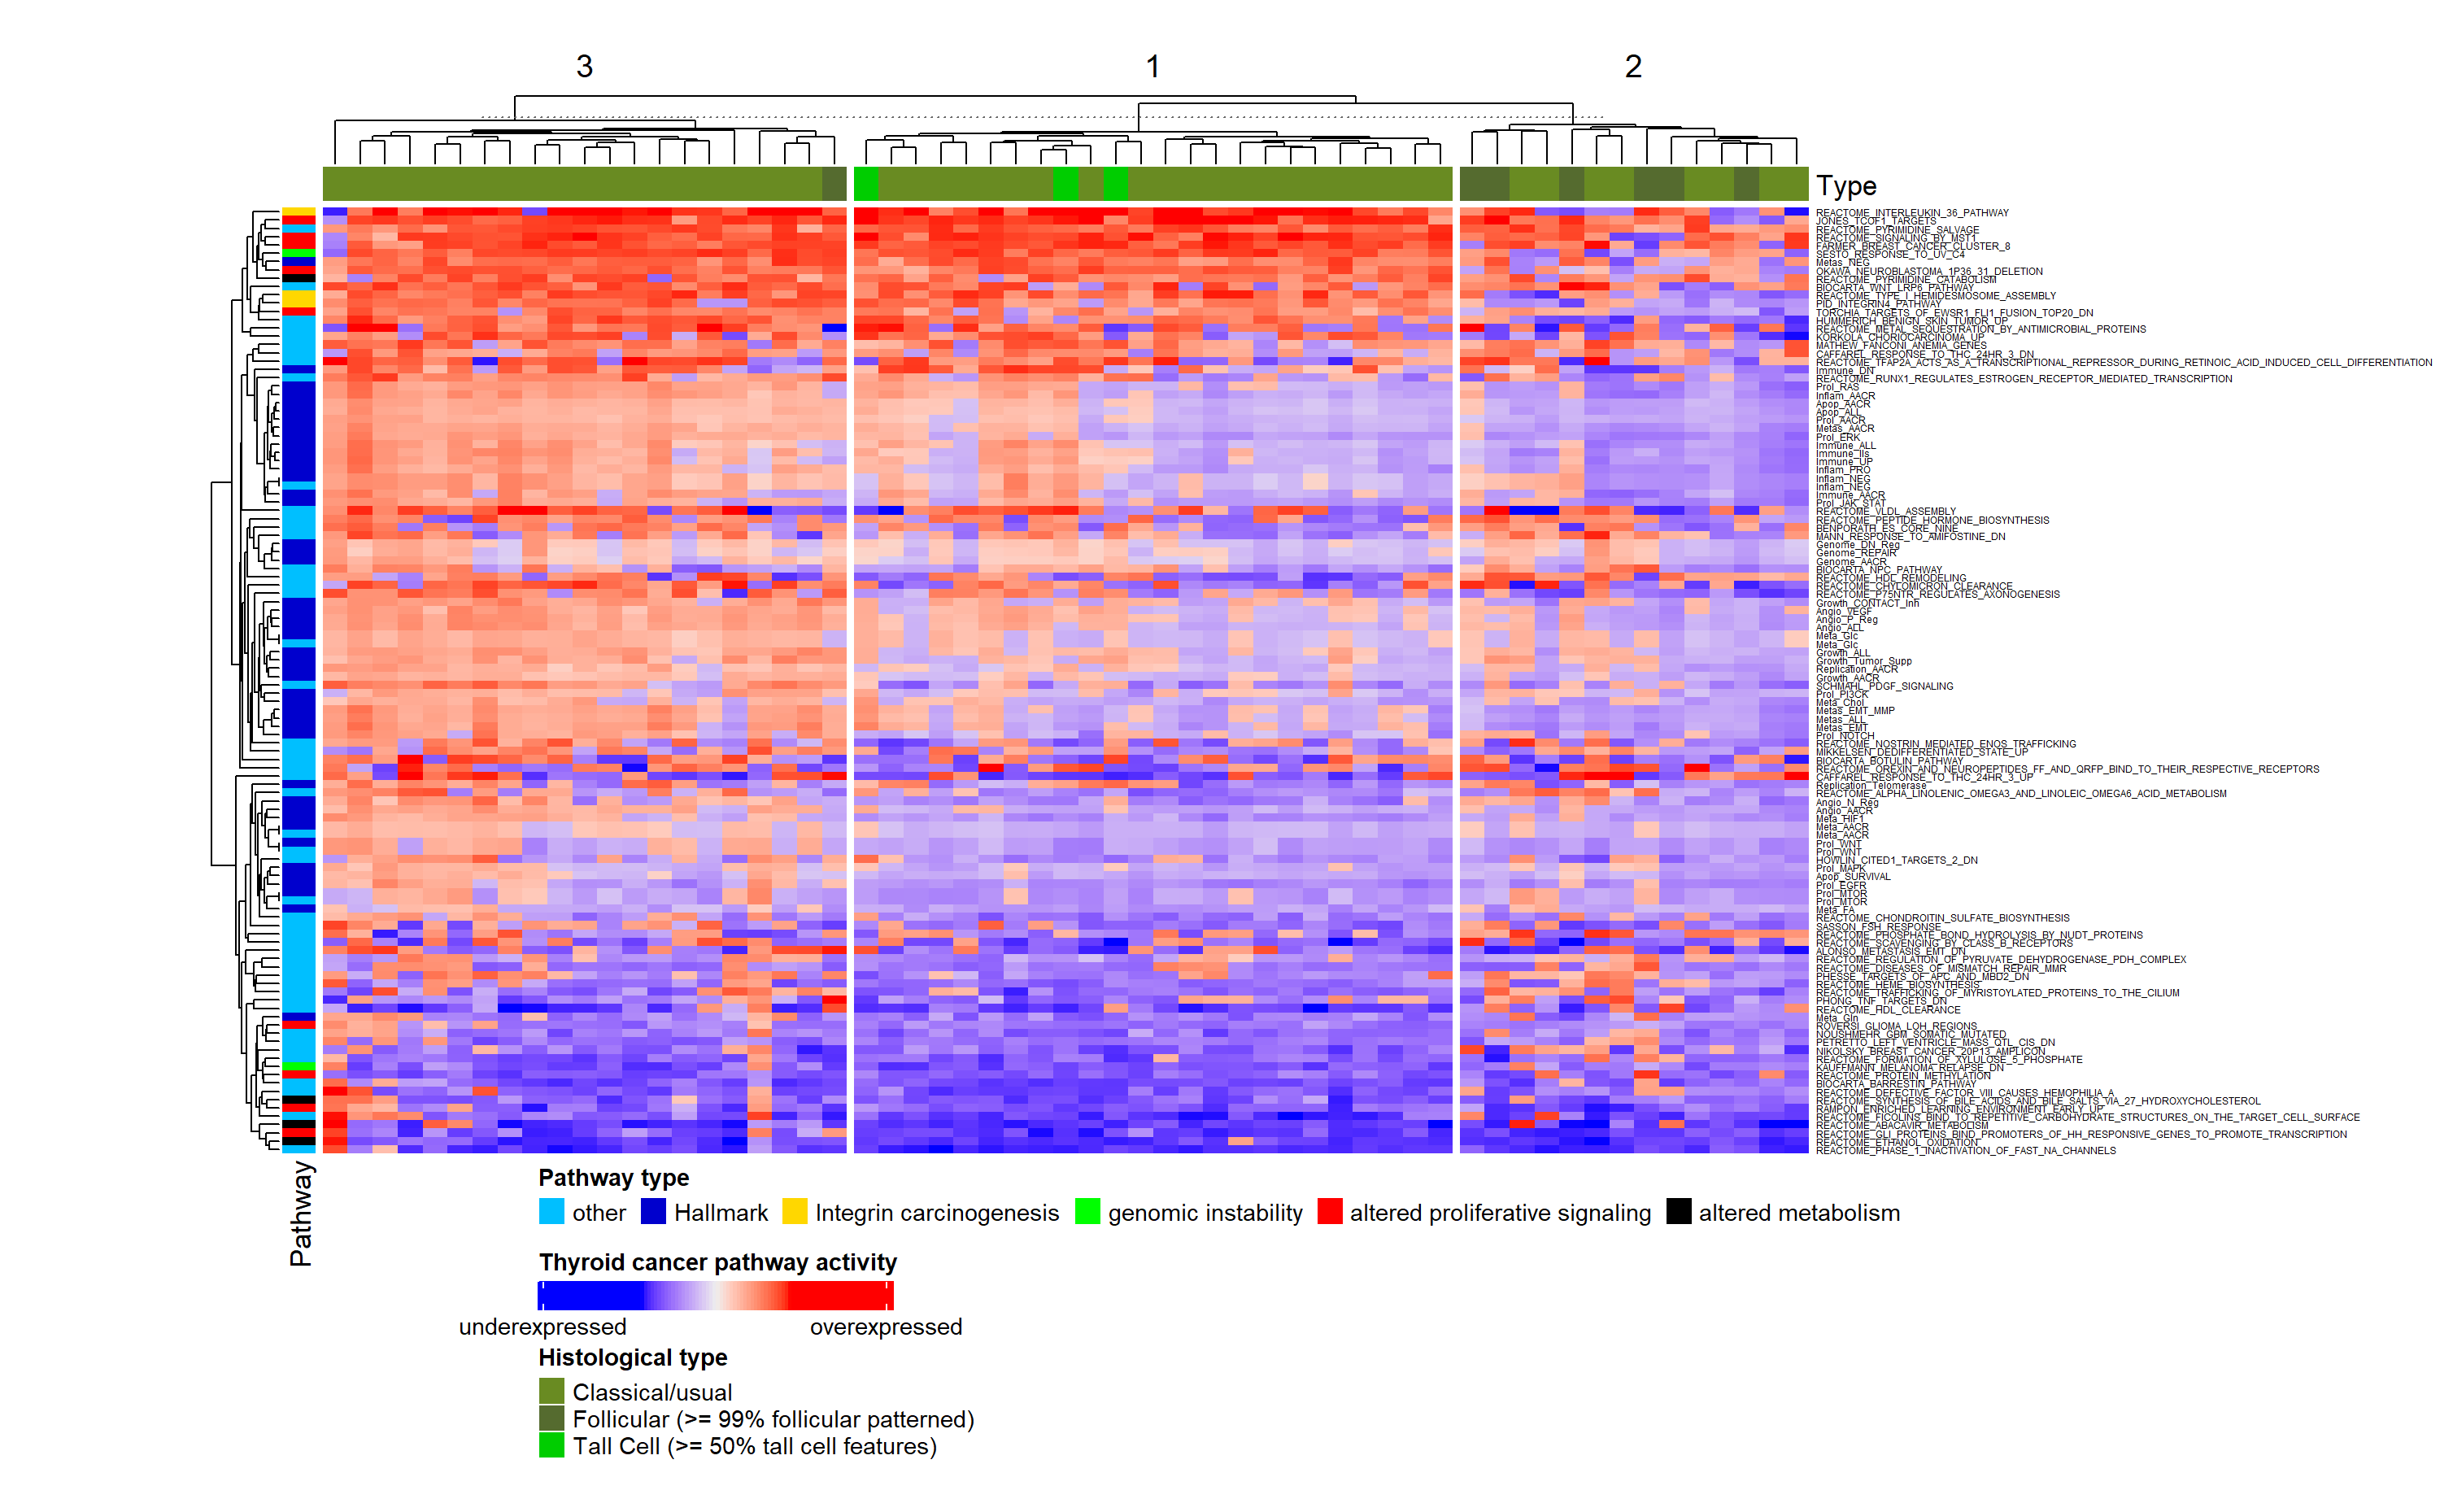
\includegraphics[width=1\linewidth]{figures/THCA GSEA Heatmap fertig top 50} 

}

\caption{\textbf{Pathway activity of the 50 most variant, hallmark, and 20 most significantly altered pathways for each patient.} Column clusters were obtained by k-means clustering with k=3. Pathway activities were computed via GSEA of THCA expression data. For all pathway activities see figure (XXX in the apendix).}\label{fig:THCAhmGSEA}
\end{figure}

\begin{figure}

{\centering 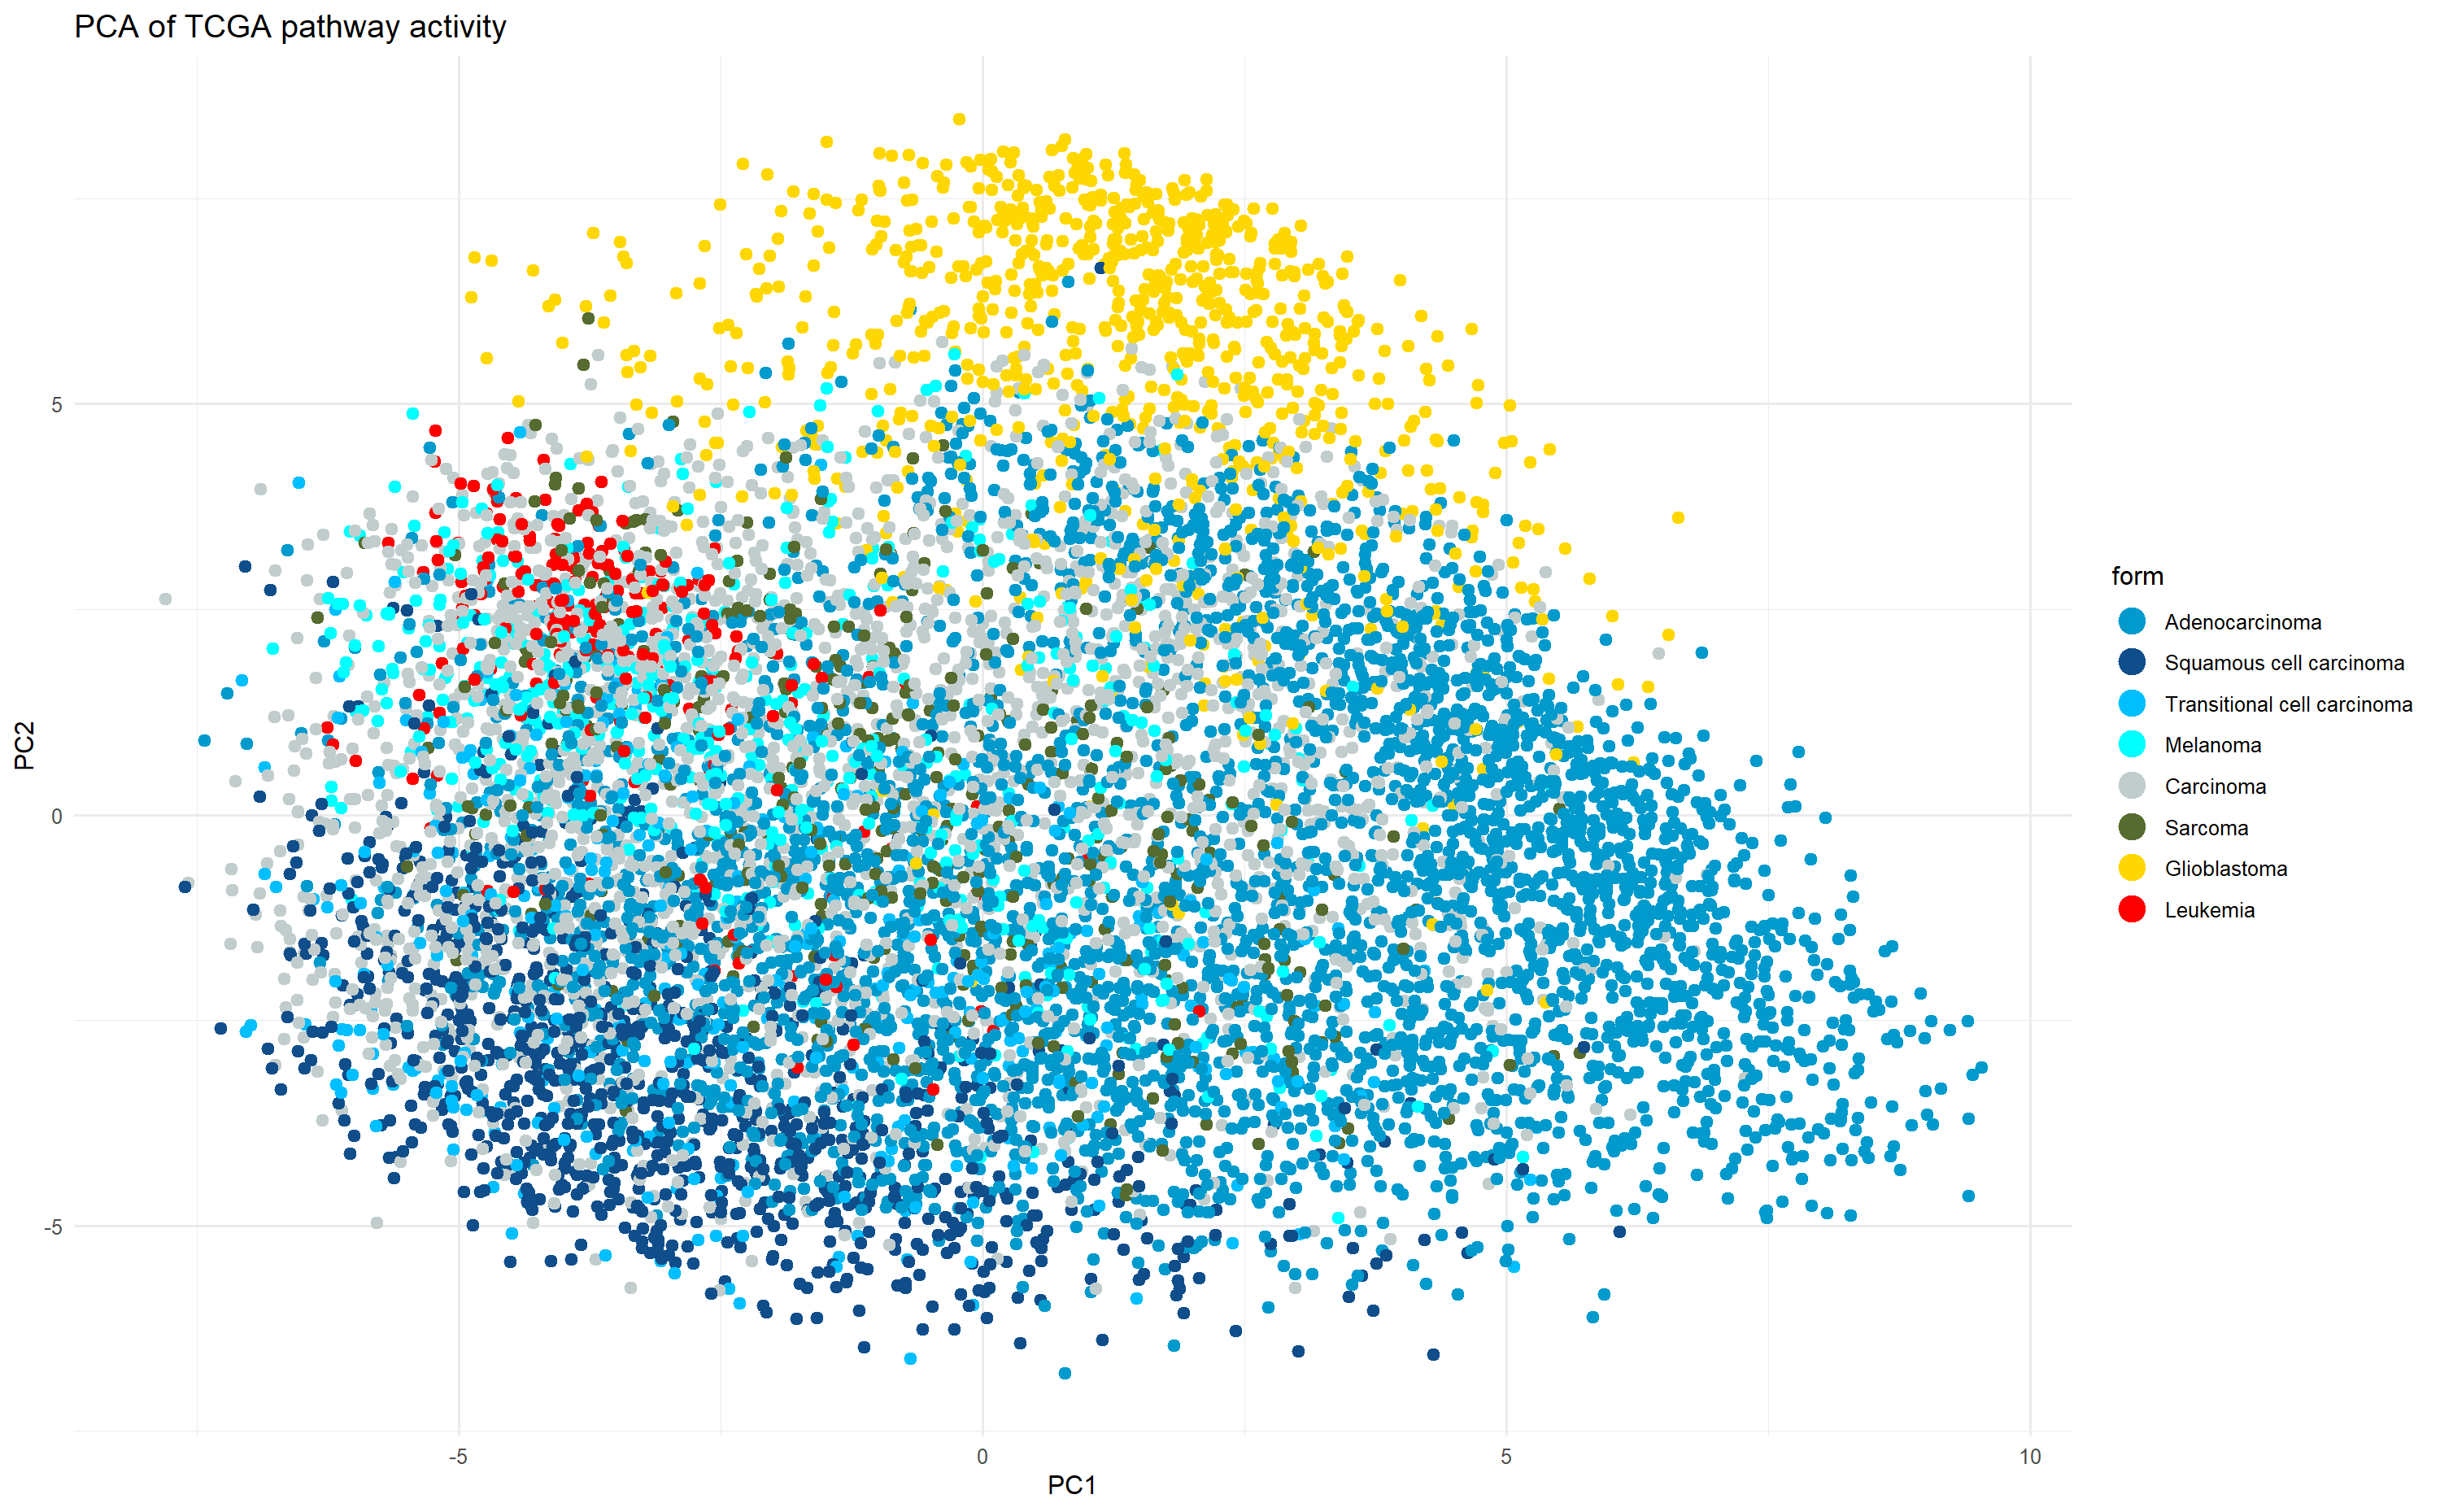
\includegraphics[width=1\linewidth]{figures/Pan Cancer PCA PC1und2 cancer form} 

}

\caption{\textbf{Results of PCA,} PC 1 and 2 are shown, samples are colored by histological type.}\label{fig:PCAcancerform}
\end{figure}

\begin{figure}

{\centering 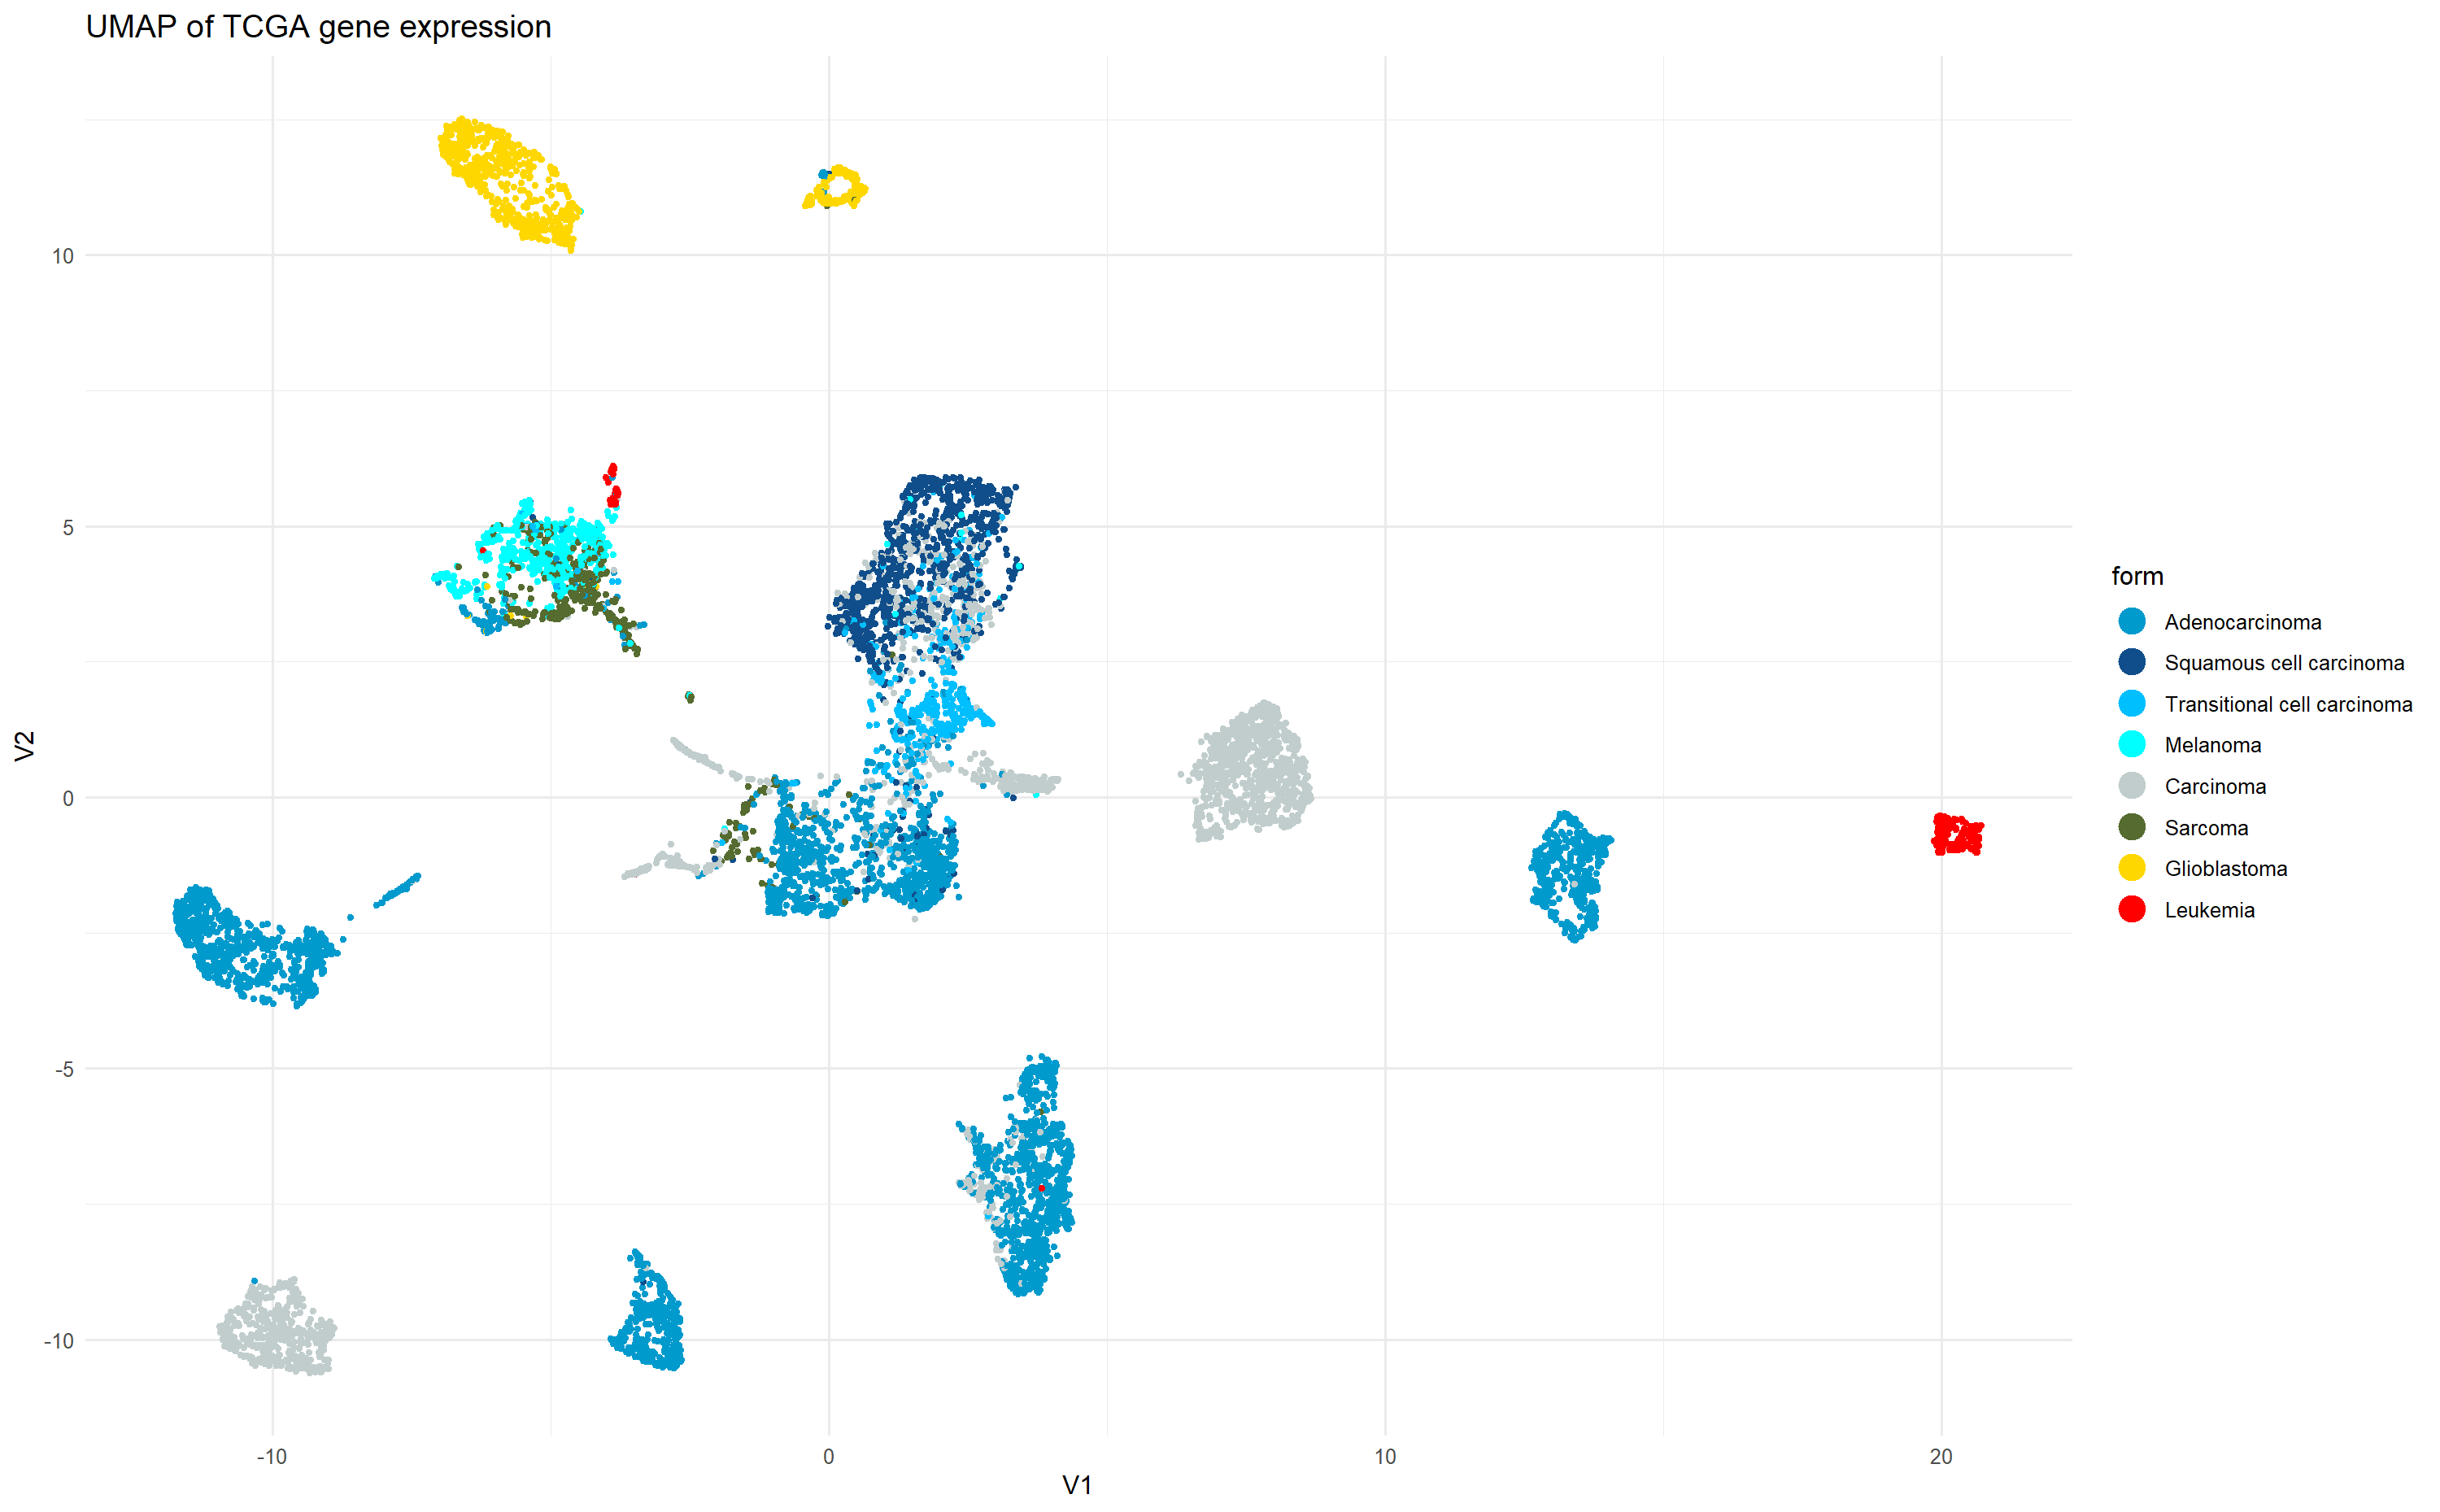
\includegraphics[width=1\linewidth]{figures/Pan Cancer Geneexpression UMAP cancer form} 

}

\caption{\textbf{UMAP performed for gene expression data,} colored by hiytological type}\label{fig:UMAPGenform}
\end{figure}

\begin{figure}

{\centering 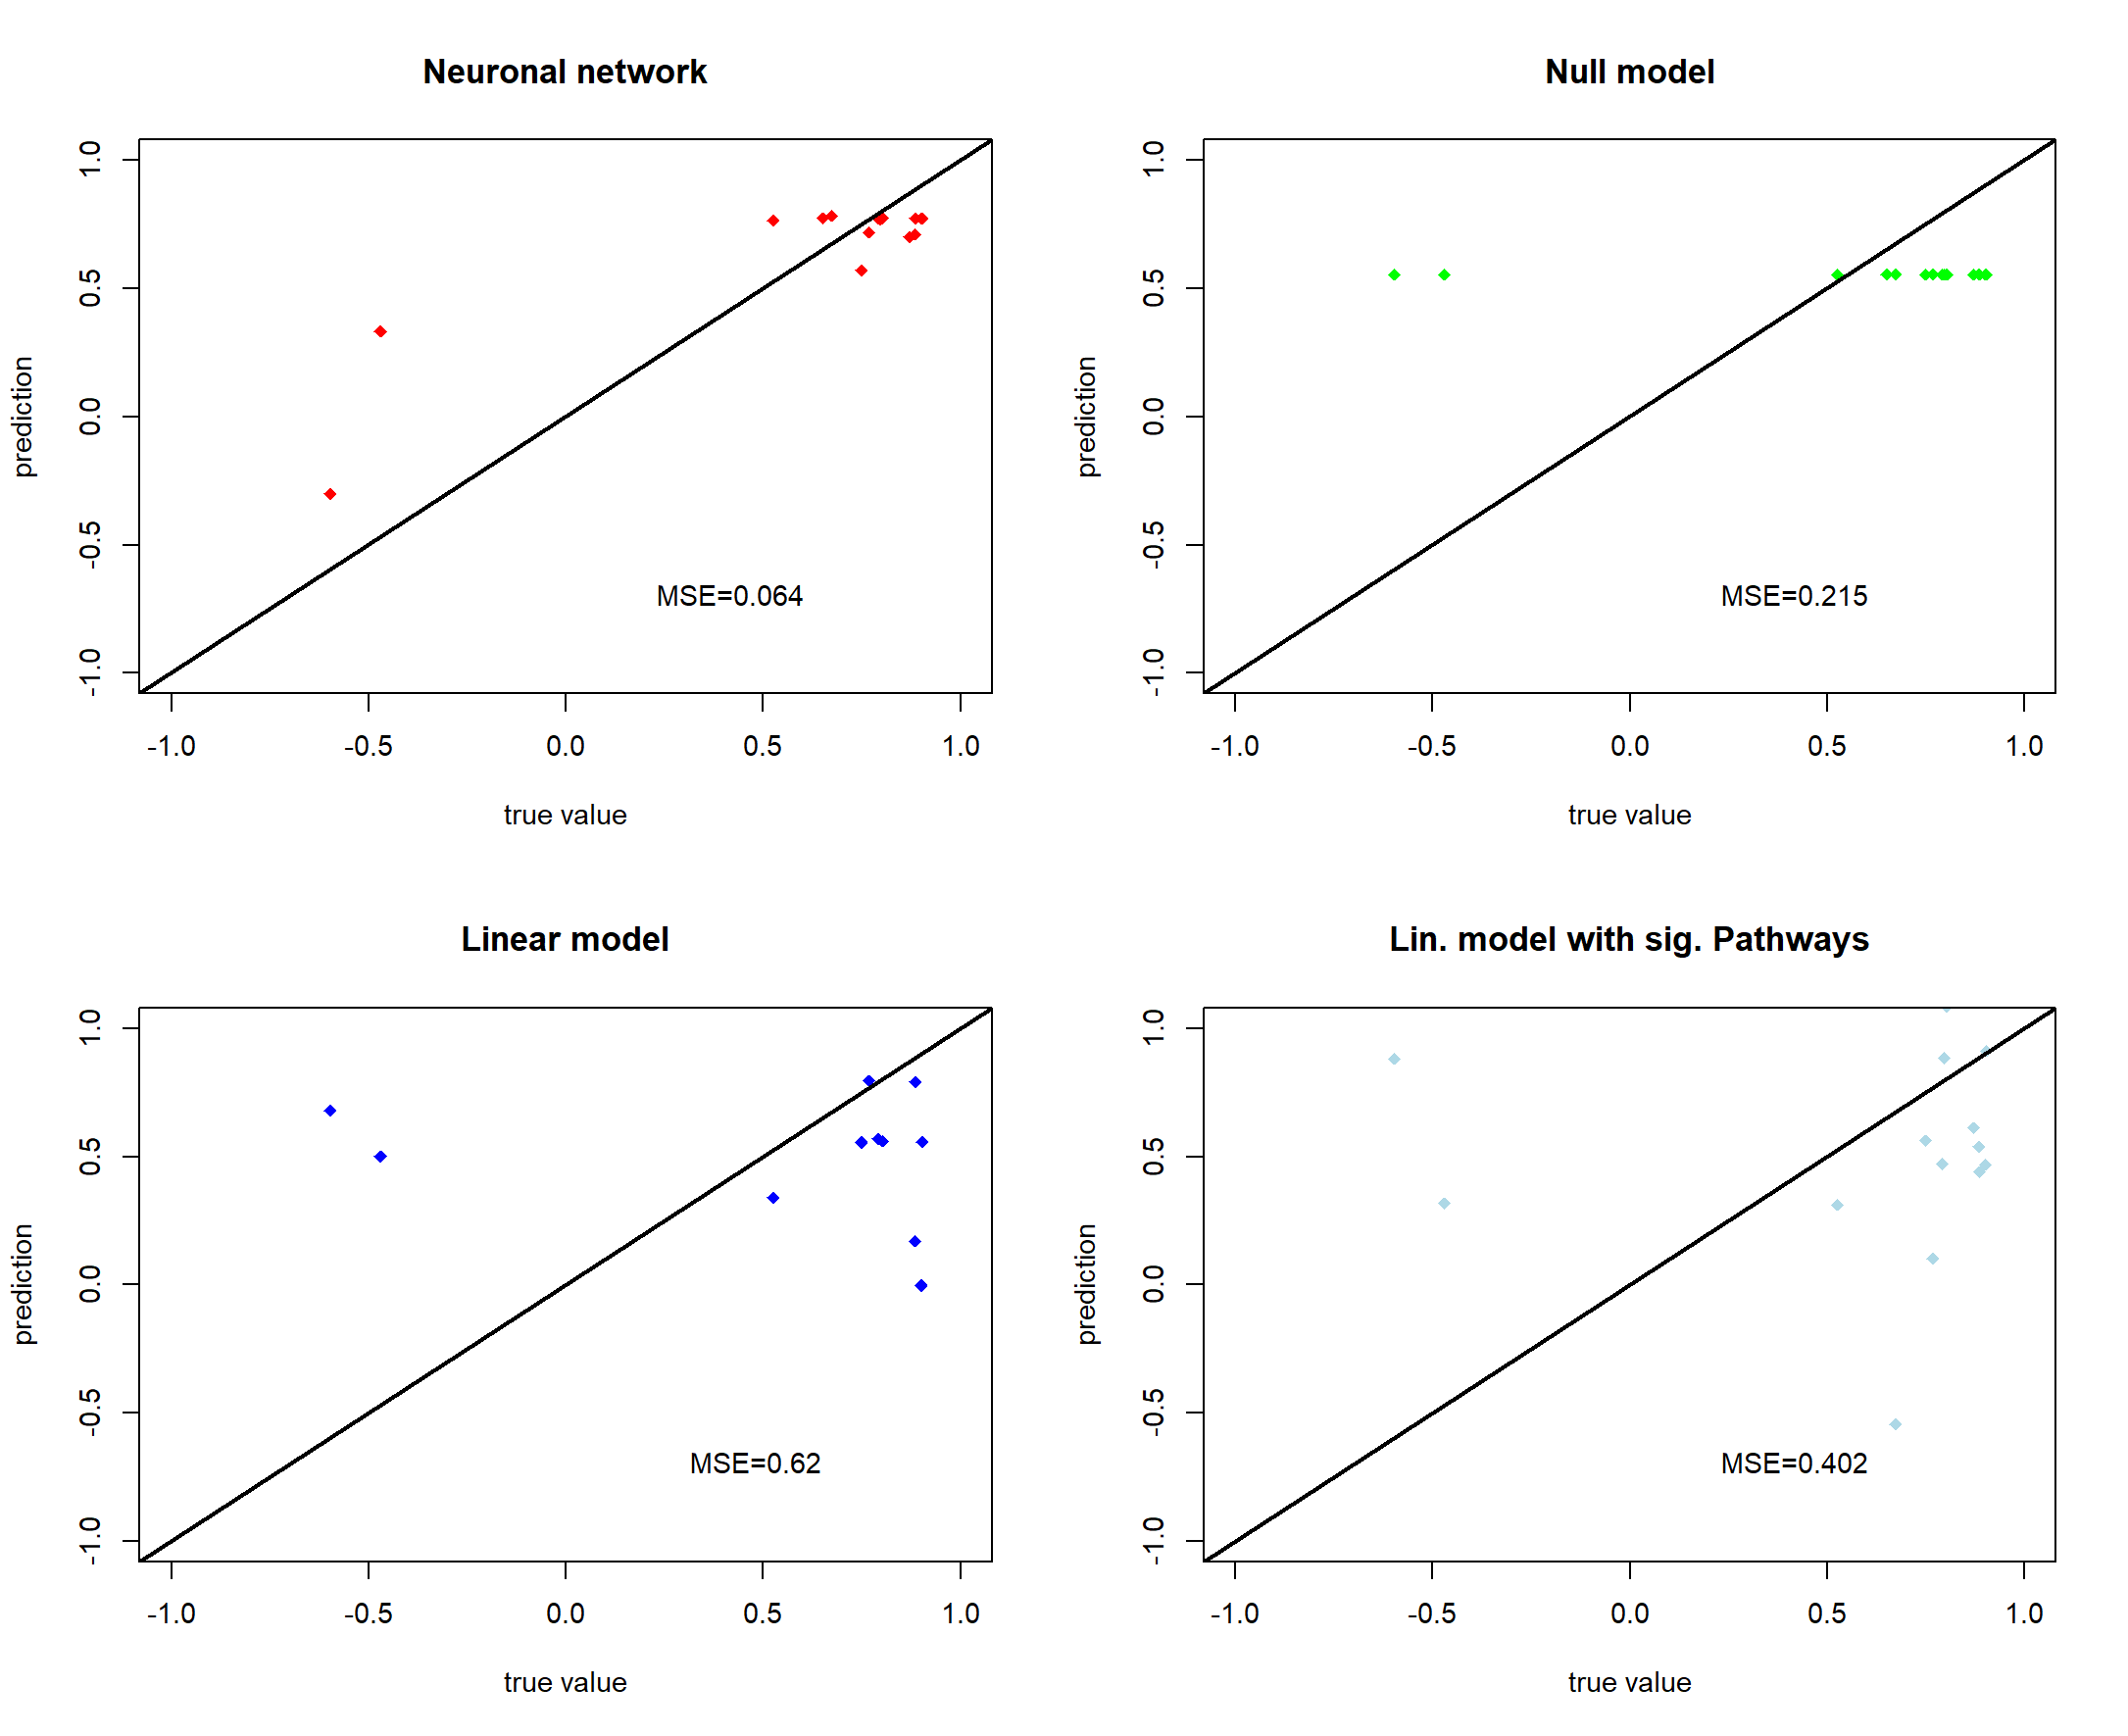
\includegraphics[width=0.8\linewidth]{figures/Regression comparison plot IL36 genes} 

}

\caption{\textbf{Regression results for various models on THCA GSEA test data.} True values are plotted against predicted values, black slope indicate a perfect prediction.}\label{fig:reg}
\end{figure}

\begin{figure}

{\centering 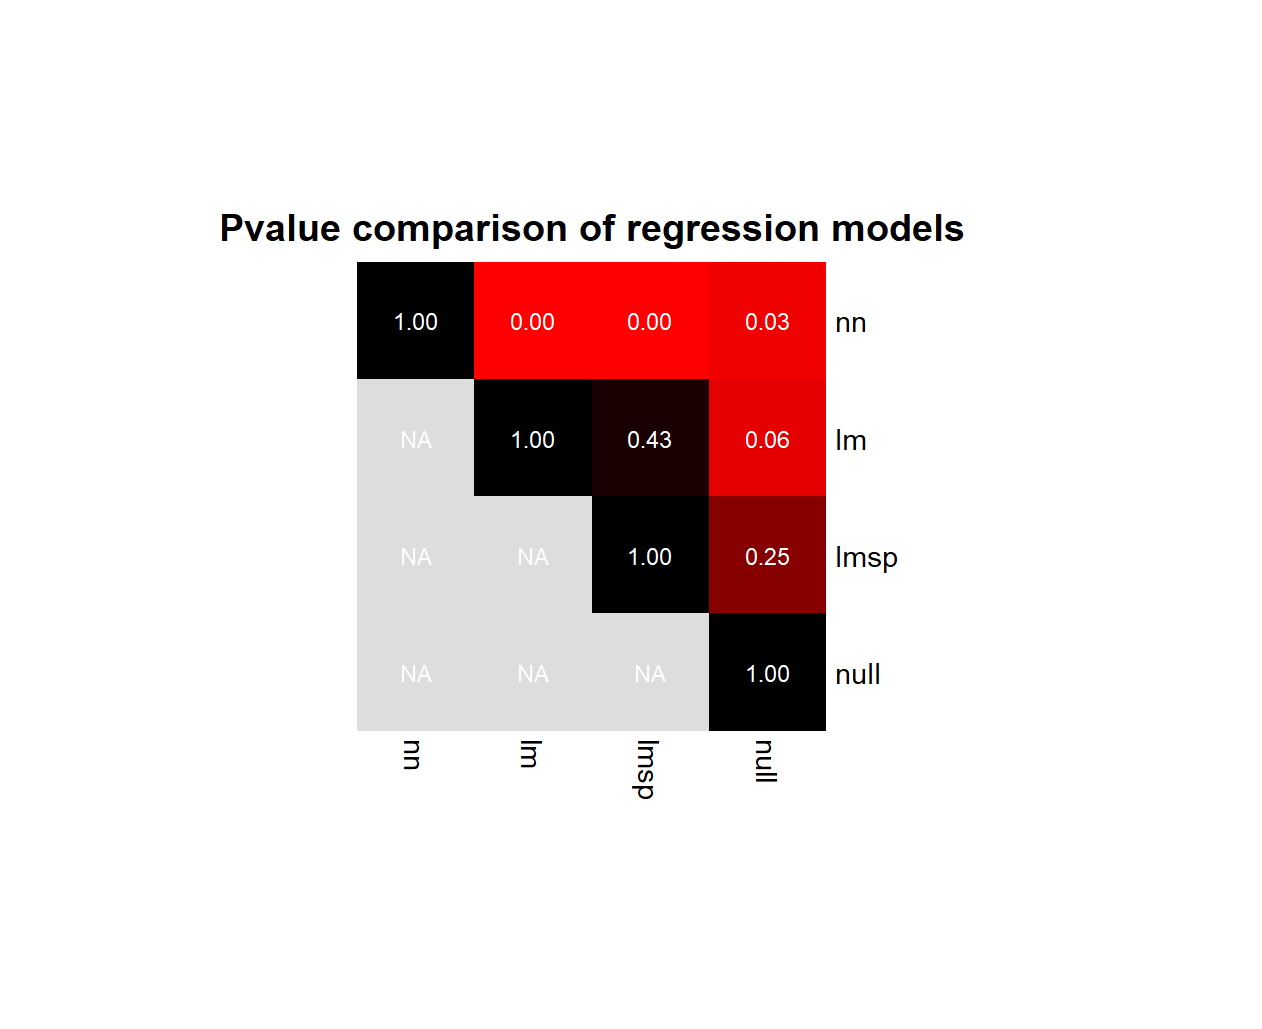
\includegraphics[width=0.3\linewidth]{figures/Regression comparison Pvalues IL36 genes} 

}

\caption{\textbf{F-test comparison of various regression models.} p-values are obtained from a two-sided variance test and displayed as heatmap. nn = neuronal network, lm = linear regression, lmsp = linear regression with only significant pathways, null = null model.}\label{fig:pval}
\end{figure}

\hypertarget{packages}{%
\section{Packages}\label{packages}}

\begin{verbatim}
## Warning: Paket 'readxl' wurde unter R Version 4.1.3 erstellt
\end{verbatim}

\begin{longtable}[]{@{}
  >{\raggedright\arraybackslash}p{(\columnwidth - 4\tabcolsep) * \real{0.14}}
  >{\raggedright\arraybackslash}p{(\columnwidth - 4\tabcolsep) * \real{0.60}}
  >{\raggedright\arraybackslash}p{(\columnwidth - 4\tabcolsep) * \real{0.26}}@{}}
\caption{Packages used in the analysis.}\tabularnewline
\toprule
\begin{minipage}[b]{\linewidth}\raggedright
Package
\end{minipage} & \begin{minipage}[b]{\linewidth}\raggedright
Usage
\end{minipage} & \begin{minipage}[b]{\linewidth}\raggedright
Authors
\end{minipage} \\
\midrule
\endfirsthead
\toprule
\begin{minipage}[b]{\linewidth}\raggedright
Package
\end{minipage} & \begin{minipage}[b]{\linewidth}\raggedright
Usage
\end{minipage} & \begin{minipage}[b]{\linewidth}\raggedright
Authors
\end{minipage} \\
\midrule
\endhead
biomart & renaming genenames to ensembleIDs & Durinck \emph{et al.,}
2009 \\
msigdbr & downloading canonical pathways and included genes from MSigDB
& Bhuva \emph{et al.,} 2022 \\
dplyr & editing of dataframes & Wickham \emph{et al.,} 2022 \\
ggplot2 & creation of plots with detailed options & Wickham \emph{et
al.,} 2022 \\
pheatmap & creation of heatmaps with detailed options & Kolde, 2019 \\
vioplot & creation of violinplots & Kolde, 2019 \\
VennDiagram & creation of VENN-diagrams & Chen, 2022 \\
fgsea & performing a GSEA & Korotkevich \emph{et al.,} 2019 \\
GSVA & performing a GSVA & Hänzelmann \emph{et al.,} 2013 \\
ComplexHeatmap & creation of heatmaps with detailed options & Gu
\emph{et al.,} 2016 \\
metaplot & creating of data-driven plots & Bergsma, 2019 \\
gridExtra & implementing of ``grid'' graphics & Auguie and Antonov,
2017 \\
umap & creating UMAPs & Konopka, 2022 \\
gage & application of GSEA & Luo \emph{et al.,} 2009 \\
psych & performing an iterative factor analysis & Revelle, 2022 \\
cluster & performing a cluster analysis & Maechler \emph{et al.,}
2022 \\
MASS & implementing of neural network & Ripley \emph{et al.,} 2022 \\
neuralnet & training of neural networks & Fritsch \emph{et al.,} 2019 \\
AnnotationDbi & translating ensemble ids into gennames & Pagès \emph{et
al.,} 2022 \\
org.Hs.eg.db & translating ensemble ids into gennames & Carlson, 2019 \\
\bottomrule
\end{longtable}

\end{document}
